
% https://deepgenerativemodels.github.io/


\newcommand{\D}{\mathcal{D}}
\newcommand{\KL}[2]{D_\mathrm{KL}\paren{#1 \mathbin{\|} #2}}
\renewcommand{\P}{\mathcal{P}}
\newcommand{\X}{\mathcal{X}}
\newcommand{\Z}{\mathcal{Z}}
\newcommand{\Q}{\mathcal{Q}}
\newcommand{\bb}{\mathbf{b}}
\newcommand{\bc}{\mathbf{c}}
\newcommand{\bh}{\mathbf{h}}
\newcommand{\bv}{\mathbf{v}}
\newcommand{\bx}{\mathbf{x}}
\newcommand{\bz}{\mathbf{z}}
\newcommand{\M}{\mathcal{B}}
\newcommand{\ELBO}{\mathrm{ELBO}}
\newcommand{\giv}{\mid}
\newcommand{\paren}[1]{\left(#1\right)}
\newcommand{\brac}[1]{\left[#1\right]}
\newcommand{\veps}{\varepsilon}
\newcommand{\set}[1]{\left\{#1\right\}}
\renewcommand{\d}{\mathop{}\!\mathrm{d}}
\newcommand{\Expect}{\mathbb{E}}
\newcommand{\Normal}{\mathcal{N}}
\newcommand{\I}{\mathbf{I}}
\newcommand{\0}{\mathbf{0}}


\chapter{Deep Generative Models}
\setcounter{section}{-1}

%+++++++++++++++++++++++++++++++++++++++++++
\section{Overview}
%-------------------------------------------
% https://deepgenerativemodels.github.io/

Generative models are widely used in many subfields of AI and Machine Learning. Recent 
advances in parameterizing these models using deep neural networks, combined with 
progress in stochastic optimization methods, have enabled scalable modeling of complex, 
high-dimensional data including images, text, and speech. In this chapter, we will 
study the probabilistic foundations and learning algorithms for deep generative models, 
including variational autoencoders, generative adversarial networks, autoregressive 
models, normalizing flow models, energy-based models, and score-based models. This 
chapter will also discuss application areas that have benefitted from deep generative 
models, including computer vision, speech and natural language processing, graph mining, 
reinforcement learning, reliable machine learning, and inverse problem solving.

Generative models are classified as unsupervised learning. In a very general way, a
generative model is one that given a number of samples (training set) drawn from a 
distribution $p(\bx)$, is capable of learning an estimate $p_g(\bx)$ of such distribution 
somehow.

There are several estimation methods on which generative models are based. However, to 
simplify their classification \cite{Goodfellow2016}, only generative models based on 
maximum likelihood will be considered.

\begin{figure}[H]
\centering
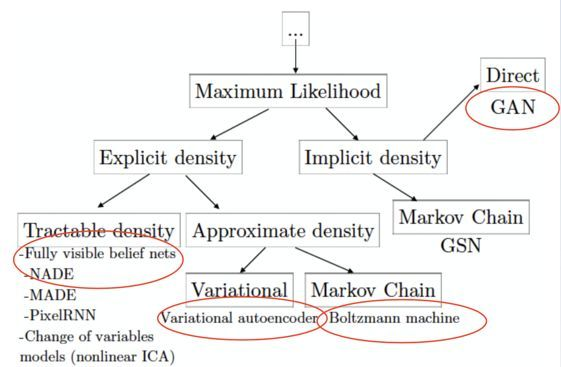
\includegraphics[scale=0.618]{pix/dgm/taxonomy_goodfellow.jpeg}
\caption{Taxonomy of generative models based on maximum likelihood. Extracted from \cite{Goodfellow2016}}
\label{fig:taxonomy_generative_models}
\end{figure}

The idea behind the maximum likelihood framework lies in modeling the approximation of 
the prior distribution of the data, which is known as the likelihood, through some 
parameters $\theta$: $p_\theta(\bx)$. Then the parameters that maximize the likelihood 
will be selected.
\begin{align}
\theta^* = \argmax_\theta \prod_{i=1}^N p_\theta(x^{(i)})
\end{align}
In practice, it is typical to maximize the log likelihood $\log p_\theta(x^{(i)})$ as 
it is less likely to suffer numeric instability when implemented on a computer.
\begin{align}
\theta^* = \argmax_\theta \sum_{i=1}^N \log p_\theta(x^{(i)})
\end{align}

If only generative models based on maximum likelyhood are considered, they can be 
classified in two groups according to how they calculate the likelihood (or an 
approximation of it): explicit density models or implicit density models. 
{\bf 基于极大似然的生成模型分为显式概率密度模型和隐式概率密度模型两种}。
The whole taxonomy tree is shown in figure \ref{fig:taxonomy_generative_models}.

Intelligent agents are constantly generating, acquiring, and processing
data. This data could be in the form of {\em images} that we capture on our
phones, {\em text} messages we share with our friends, {\em graphs} that model
interactions on social media, {\em videos} that record important events,
etc. Natural agents excel at discovering patterns, extracting
knowledge, and performing complex reasoning based on the data they observe. How
can we build artificial learning systems to do the same?

生成模型能够从训练集中学习数据分布。学到数据分布之后,就可以生成新的数据样本。如下图 \ref{fig:dgm_generating_data} 所示,
给定一个二维点集,假设它是由一个随机变量生成出来的。假设这个随机变量服从正态分布 $p(z)$。
根据观测到的数据点,能够估计正态分布的均值和方差。知道 $p(z)$ 之后,可以根据 $p(z)$ 
来生成一些新的数据点。

\begin{figure}[H]
\centering
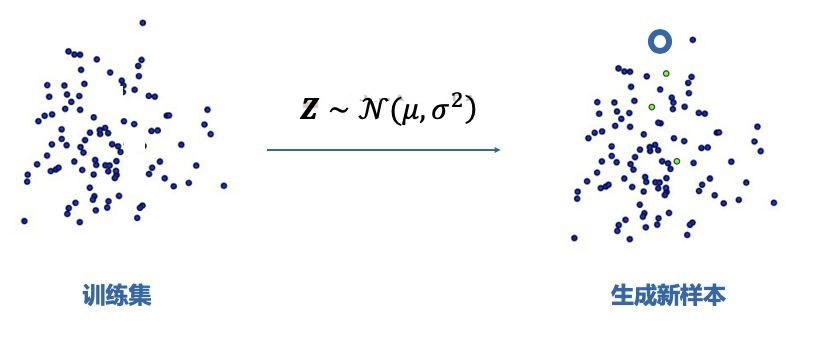
\includegraphics[scale=0.618]{pix/dgm/generating_data.jpeg}
\caption{Learning and generating}
\label{fig:dgm_generating_data}
\end{figure}

我们可以将这个例子进行拓展,将 $\bz$ 看作一幅图像或者自然语言的句子。比如把 $\bz$ 
想象成一幅图像。给定观测到的手写数字的图像集合,可以尝试学习手写数字图像的分布 $p(\bz)$。
然后根据 $p(\bz)$ 的采样,来生成下图\ref{fig:dgm_digital_numbers}右边所示的图像。在这个例子中,
生成模型主要做的事情是抓住手写数字图像的结构,以生成的类似的图像。

\begin{figure}[H]
\centering
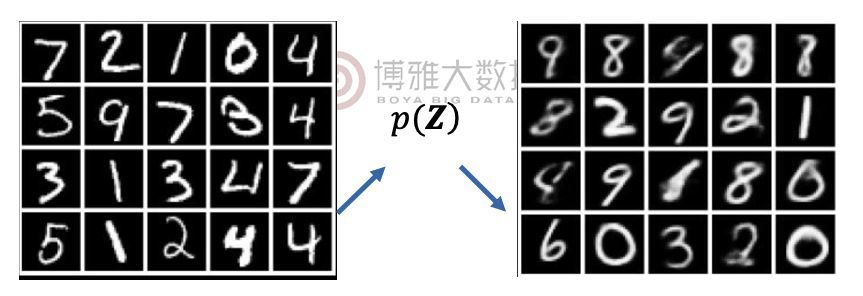
\includegraphics[scale=0.618]{pix/dgm/hand_writn_digitals.jpeg}
\caption{hand-written digital numbers}
\label{fig:dgm_digital_numbers}
\end{figure}


In this chapter, we will study generative models that view the world under the lens of probability.
In such a worldview, we can think of any kind of
observed data, say $\mathcal{D}$, as a finite set of samples from an
underlying distribution, say $p_{\mathrm{data}}$. At its very core, the
goal of any generative model is then to approximate this data
distribution given access to the dataset $\mathcal{D}$. The hope is that
if we are able to {\em learn} a good generative model, we can use the
learned model for downstream {\em inference}.


%+++++++++++++++++++++++++++++++++++++++++++
\subsection{Explicit Density Models}

Explicit density models can be subdivided in two types: those capable of directly 
maximizing an explicit density $p_\theta(\bx)$ and those capable of maximizing an 
approximation of it. This subdivision represents two different ways of dealing with 
the problem of tractability when maximizing the likelihood. Some of the most famous 
approaches to tractable density models are Pixel Recurrent Neural Networks 
(PixelRNN) [12] and Nonlinear Independent Components Analysis (NICA) [13].
The models that maximize an approximation of the density function $p_\theta(\bx)$ 
are likewise subdivided into two categories depending on whether the approximation 
is deterministic or stochastic: variational or Markov chain. Later in this chapter 
the most widely approach to variational learning, the variational autoencoder also 
known as VAE will be analyzed in detail (see Section 3 and Section 4).
Furthermore, Section 2.2 describes one of the simplest explicit density models, 
Probabilistic PCA, and serves as an introduction to this type of models.


%+++++++++++++++++++++++++++++++++++++++++++
\subsection{Implicit Density Models}

These are models that do not estimate the density probability but instead define a 
stochastic procedure which directly generates data [14]. This procedure involves 
comparing real data with generated data. Some of the most famous approaches are 
the Generative Stochastic Network [15] and Generative Adversarial Network [16].


%+++++++++++++++++++++++++++++++++++++++++++
\subsection{Learning}

We will be primarily interested in parametric approximations to the data
distribution, which summarize all the information about the dataset $\mathcal{D}$ in
a finite set of parameters. In contrast with non-parametric models,
parametric models scale more efficiently with large datasets but are
limited in the family of distributions they can represent.

In the parametric setting, we can think of the task of learning a
generative model as picking the parameters within a family of model
distributions that minimizes some notion of distance\footnote{
  As we shall see later, functions that do not satisfy all 
  properties of a distance metric are also used in practice, e.g., KL
  divergence.} 
between the model distribution and the data distribution.

%\begin{comment}
\begin{figure}[H]
	\centering
	\begin{minipage}{0.49\linewidth}
		\centering
		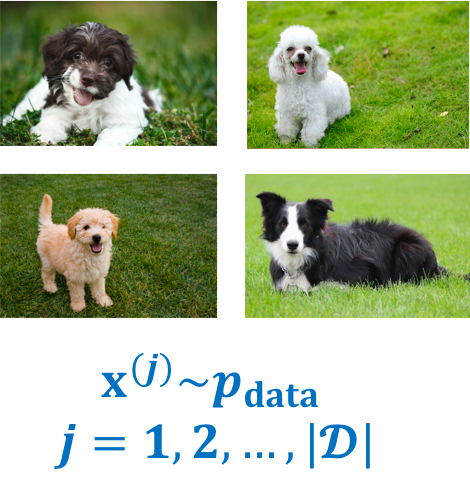
\includegraphics[scale=0.518]{pix/dgm/learning_1.png}
	\end{minipage}
	%\qquad
	\begin{minipage}{0.49\linewidth}
		\centering
		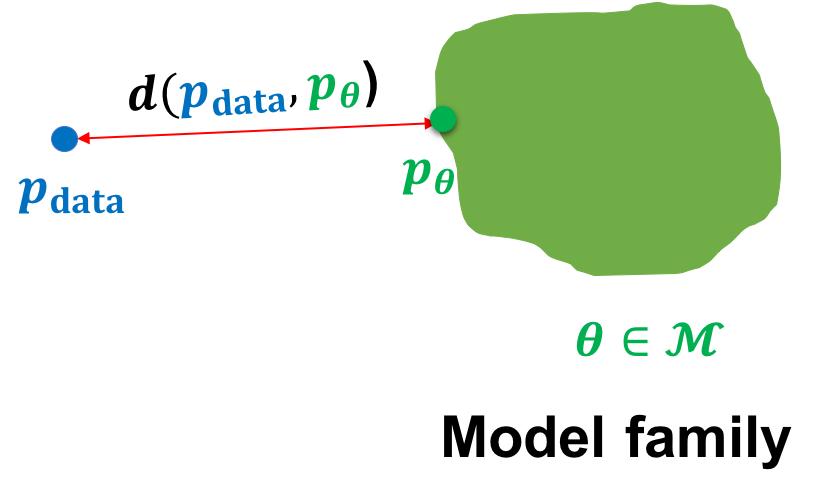
\includegraphics[scale=0.518]{pix/dgm/learning_2.png}
	\end{minipage}
\end{figure}
%\end{comment}

For instance, we might be given access to a dataset of dog images $\mathcal{D}$ and
our goal is to learn the parameters of  a generative model $\theta$ within a model 
family $\mathcal{M}$ such that
the model distribution $p_\theta$ is close to the data distribution over dogs
$p_{\mathrm{data}}$. Mathematically, we can specify our goal as the
following optimization problem: 
\begin{equation}
\min_{\theta\in \mathcal{M}}d(p_{\mathrm{data}}, p_{\theta})
\label{eq:learning_gm}
%\tag{1}
\end{equation}
where $p_{\mathrm{data}}$ is accessed via the dataset
$\mathcal{D}$ and $d(\cdot)$ is a notion of distance between probability distributions.

As we navigate through this chapter, it is interesting to take note of
the difficulty of the problem at hand. A typical image from a modern
phone camera has a resolution of approximately $700 \times 1400$ pixels.
Each pixel has three channels: R(ed), G(reen) and B(lue) and each
channel can take a value between $0$ to $255$. Hence, the number of possible
images is given by $256^{700 \times 1400 \times 3}\approx 10 ^{800000}$.
In contrast, ImageNet, one of the largest publicly available datasets,
consists of only about 15 million images. Hence, learning a generative
model with such a limited dataset is a highly underdetermined problem.

Fortunately, the real world is highly structured and automatically
discovering the underlying structure is key to learning generative
models. For example, we can hope to learn some basic artifacts about
dogs even with just a few images: two eyes, two ears, fur etc. Instead
of incorporating this prior knowledge explicitly, we will hope the model
learns the underlying structure directly from data. There is no free
lunch however, and indeed successful learning of generative models will
involve instantiating the optimization problem in
$(\ref{eq:learning_gm})$ in a suitable way. In this chapter, we will be
primarily interested in the following questions:

\begin{itemize}
%\setlength{\itemsep}{0pt}
%\setlength{\parsep}{0pt}
\setlength{\parskip}{0pt}
\item[-]
What is the representation for the model family $\mathcal{M}$?

\item[-]
What is the objective function $d(\cdot)$?

\item[-]
What is the optimization procedure for minimizing $d(\cdot)$?
\end{itemize}

In the next few sections, we will take a deeper dive into certain
families of generative models. For each model family, we will note how
the representation is closely tied with the choice of learning objective
and the optimization procedure.


%+++++++++++++++++++++++++++++++++++++++++++
\subsection{Inference}

For a discriminative model such as logistic regression, the fundamental
inference task is to predict a label for any given datapoint. Generative
models, on the other hand, learn a joint distribution over the entire
data.\footnote{Technically, a probabilistic discriminative model is also a
    generative model of the labels conditioned on the data. However, the
    usage of the term generative models is typically reserved for high
    dimensional data.}

While the range of applications to which generative models have been
used continue to grow, we can identify three fundamental inference
queries for evaluating a generative model.:

\begin{itemize}
%\setlength{\itemsep}{0pt}
%\setlength{\parsep}{0pt}
\setlength{\parskip}{0pt}
\item[1.]
{\bf Density estimation:} Given a datapoint $\mathbf{x}$, what is the
    probability assigned by the model, i.e., $p_\theta(\mathbf{x})$?

\item[2.]
{\bf Sampling:} How can we {\bf generate} novel data from the model
    distribution, i.e.,
    $\mathbf{x}_{\mathrm{new}} \sim p_\theta(\mathbf{x})$?

\item[3.]
{\bf Unsupervised representation learning:} How can we learn meaningful
    feature representations for a datapoint $\mathbf{x}$?
\end{itemize}

Going back to our example of learning a generative model over dog
images, we can intuitively expect a good generative model to work as
follows. For density estimation, we expect $p_\theta(\mathbf{x})$ to be
high for dog images and low otherwise. Alluding to the name {\bf generative
model}, sampling involves generating novel images of dogs beyond the
ones we observe in our dataset. Finally, representation learning can
help discover high-level structure in the data such as the breed of
dogs.

In light of the above inference tasks, we note two caveats. First,
quantitative evaluation of generative models on these tasks is itself
non-trivial (in particular, sampling and representation learning) and an
area of active research. Some quantitative metrics exist, but these
metrics often fail to reflect desirable qualitative attributes in the
generated samples and the learned representations. Secondly, not all
model families permit efficient and accurate inference on all these
tasks. Indeed, the trade-offs in the inference capabilities of the
current generative models have led to the development of very diverse approaches as
we shall see in this course.


%+++++++++++++++++++++++++++++++++++++++++++
\section{Energy Based Model(EBM)}
%-------------------------------------------


%+++++++++++++++++++++++++++++++++++++++++++
\subsection{基于能量的模型}

基于能量的模型中常用的一个概率分布是玻尔兹曼分布,其概率密度函数形式如下:
\begin{align*}
p(z) = \frac{e^{-E(z)}}{\Sigma_z e^{-E(z)}}
\end{align}
其中 $E(z)$ 为能量函数,$\Sigma_z e^{-E(z)}$ 为配分函数或归一化常数。

当一个事件发生的概率最大的时候,能量最低。例如自然界中的一些事物或者物质,其实是处于低能态,
因为高能态的东西不太稳定。所以要使得 $E(z)$ 比较小的时候,概率密度比较大。

在基于能量的模型(EBM)中还要加入隐变量来刻画数据生成。为了便于描述,我们将上述 $z$ 改记为 
$x$。比如假设 $\mathcal{F}(z)$ 包含隐变量 $h$:
$$
\mathcal{F}(x) = -\log \Sigma_h e^{-\mathbb{E}(x,h)}
$$
在物理学中 $\mathcal{F}(x)$ 称为自由能。
所以 $p(x)$ 可以写成包含隐变量 $h$ 的联合概率密度函数:
\begin{align*}
p(x) =& \sum_h \underset{\textcolor{blue}{\downarrow}}{p(x,h)}
= \underset{\textcolor{red}{\downarrow}}{\frac{1}{Z}} \sum_h e^{-\mathbb{E}(x,h)}
= \frac{1}{Z} e^{-\underset{\textcolor{blue}{\downarrow}}{\mathcal{F}(x)}} \\
&\qquad
\textcolor{blue}{\text{隐变量}}
\quad
\textcolor{red}{Z = \sum_x e^{-\mathcal{F}(x)}}
\qquad\quad
\textcolor{blue}{\text{自由能}}
\end{align}
已知 $p(x)$ 的形式后,可以使用极大似然估计来学习参数。下面说明如何使用 MLE 来训练 EBM。给定 
$n$ 个训练样本,将似然函数作为优化目标,其数学表达式为:
$$
L(\theta) = \prod_{i=1}^n p(x_i; \theta)
$$
优化的目标函数为:
$$
l(\theta) = \frac{1}{n}\log L(\theta)
= \frac{1}{n}\sum_i\log\frac{ e^{-\mathcal{F}(x_i)} }{Z}
= \frac{1}{n}\sum_i\left( \mathcal{F}(x_i) + \log Z \right)
$$
然后用梯度下降法来求解。注意配分函数 $\log Z$ 包含参数信息,不能忽略。关于怎样求解这个东西,简单来说,
因为 $Z$ 涉及高维积分,求导时我们需要对模型进行一些采样。


%+++++++++++++++++++++++++++++++++++++++++++
\subsection{Boltzmann Machine}

基于能量的模型的一个典型例子是 Boltzmann Machine。它其实是一个物理概念。一般而言,
能量函数为某周特殊形式的基于能量的模型,称为 Boltzmann Machine:
$$
p(x) = \frac{e^{-\mathbb{E}(x)}}{Z}
$$
Boltzmann Machine 是联合概率分布模型。在 Boltzmann Machine 中,能量函数是观测数据变量的一个二次函数:
\begin{align*}
&\quad
\textcolor{blue}{\text{参数矩阵}} \\
\mathbb{E}(\bx)=& -\bx^T \overset{\textcolor{blue}{\downarrow}}{U} \bx 
- \underset{\textcolor{blue}{\uparrow}}{\bb^T} \bx \\
&\qquad\qquad 
\textcolor{blue}{\text{偏置向量}}
\end{align}
其中 $U$ 是参数矩阵,$\bb$ 是偏置向量。根据训练数据学习模型,主要是估计参数 $U$
 和 $\bb$。玻尔兹曼机是一个多维联合概率分布,极大似然估计可以解决学习的问题。

假设 $v$ 为观测变量(observed variable),玻尔兹曼机里还可以加入一些隐变量(latent variable) 
$h$。此时能量函数同样也是二次函数,但是此时还包含交叉项。例如,观测变量 $v$ 和隐变量 $h$ 
之间的交叉项,还有隐变量与隐变量之间的二次项、偏置变量。

Boltzmann Machine with latent elements:
\begin{itemize}
%\setlength{\itemsep}{0pt}
%\setlength{\parsep}{0pt}
\setlength{\parskip}{0pt}
\item[-]
原始变量 $\bx$ 变成为 observed variable $\bv$ 和 latent variable $\bh$ 两部分

\item[-]
拟合变量之间的非线性关系

\item[-]
近似任意的离散变量的概率质量函数(probability mass function)

\item[-]
能量函数可以改写为:
$$
\mathbb{E}(\bv, \bh) = \bv^T R \bv - \bv^T W \bh - \bh^T S \bh - \bb^T \bv - \bc^T \bh
$$
\end{itemize}


%+++++++++++++++++++++++++++++++++++++++++++
\section{Autoregressive Models}
%-------------------------------------------

We begin our study into generative modeling with autoregressive models. As before, 
we assume we are given access to a dataset $\mathcal{D}$ of $n$-dimensional 
datapoints $\mathbf{x}$. For simplicity, we assume the datapoints are binary, i.e., 
$\mathbf{x} \in \{0,1\}^n$.


%+++++++++++++++++++++++++++++++++++++++++++
\subsection{Representation}

By the chain rule of probability, we can factorize the joint distribution over the 
$n$-dimensions as 
\begin{equation}
\label{eq:chain_rule}
p(\mathbf{x}) = \prod\limits_{i=1}^{n}p(x_i \vert x_1, x_2, \ldots, x_{i-1}) = 
\prod\limits_{i=1}^{n} p(x_i \vert \mathbf{x}_{< i } )
\end{equation}
where $\mathbf{x}_{< i}=[x_1, x_2, \ldots, x_{i-1}]$ denotes the vector of random 
variables with index less than $i$. 

The chain rule factorization can be expressed graphically as a Bayesian network.

\begin{figure}[H]
\centering
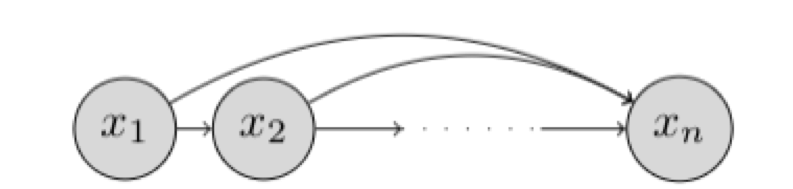
\includegraphics[scale=0.8]{pix/dgm/autoregressive.png}
\caption{Graphical model for an autoregressive Bayesian network with no 
conditional independence assumptions.}
%\label{fig:label}
\end{figure}

Such a Bayesian network that makes no conditional independence assumptions is said 
to obey the *autoregressive* property.

The term {\bf autoregressive} originates from the literature on time-series models 
where observations from the previous time-steps are used to predict the value at 
the current time step. Here, we fix an ordering of the variables $x_1, x_2, \ldots, 
x_n$ and the distribution for the $i$-th random variable depends on the values of 
all the preceding random variables in the chosen ordering $x_1, x_2, \ldots, x_{i-1}$.

If we allow for every conditional $p(x_i \vert \mathbf{x}_{< i})$ to be specified 
in a tabular form, then such a representation is fully general and can represent 
any possible distribution over $n$ random variables. However, the space complexity 
for such a representation grows exponentially with $n$.

To see why, let us consider the conditional for the last dimension, given by 
$p(x_n \vert \mathbf{x}_{< n})$. In order to fully specify this conditional, we need 
to specify a probability distribution for each of the $2^{n-1}$ configurations of 
the variables $x_1, x_2, \ldots, x_{n-1}$. For any one of the $2^{n-1}$ possible 
configurations of the variables, the probabilities should sum to one. Therefore, we 
need only one parameter for each configuration, so the total number of parameters 
for specifying this conditional is given by $2^{n-1}$. Hence, a tabular 
representation for the conditionals is impractical for learning the joint 
distribution factorized via chain rule in (\ref{eq:chain_rule}).

In an {\bf autoregressive generative model}, the conditionals are specified as 
parameterized functions with a fixed number of parameters. That is, we assume the 
conditional distributions $p(x_i \vert \mathbf{x}_{<i})$ to correspond to a Bernoulli 
random variable and learn a function that maps the preceding random variables 
$x_1, x_2, \ldots, x_{i-1}$ to the mean of this distribution. Hence, we have
$$
p_{\theta_i}(x_i \vert \mathbf{x}_{< i}) = \mathrm{Bern}(f_i(x_1, x_2, \ldots, x_{i-1}))
$$
where $\theta_i$ denotes the set of parameters used to specify the mean function 
$f_i: \{0,1\}^{i-1}\rightarrow [0,1]$. The term \textit{autoregressive} originates from 
the literature on time-series models where observations from the previous time-steps are 
used to predict the value at the current time step. Here, we are predicting the 
distribution for the $i$-th random variable using the values of the preceeding random 
variables in the sequence $x_1, x_2, \ldots, x_n$.

The number of parameters of an autoregressive generative model are given by 
$\sum_{i=1}^n \vert \theta_i \vert$. As we shall see in the examples below, the number 
of parameters are much fewer than the tabular setting considered previously. Unlike the 
tabular setting however, an autoregressive generative model cannot represent all 
possible distributions. Its expressiveness is limited by the fact that we are limiting 
the conditional distributions to correspond to a Bernoulli random variable with the 
mean specified via a restricted class of parameterized functions.

\begin{figure}[H]
\centering
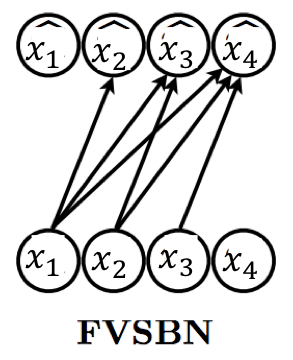
\includegraphics[scale=0.618]{pix/dgm/fvsbn.png}
\caption{A fully visible sigmoid belief network over four variables. \\ The conditionals 
are denoted by \(\widehat{x}_1, \widehat{x}_2, \widehat{x}_3, \widehat{x}_4\) 
respectively.}
%\label{fig:label}
\end{figure}
In the simplest case, we can specify the function as a linear combination of the input 
elements followed by a sigmoid non-linearity (to restrict the output to lie between 0 
and 1). This gives us the formulation of a \textit{fully-visible sigmoid belief network} 
(\href{https://papers.nips.cc/paper/1153-does-the-wake-sleep-algorithm-produce-good-density-estimators.pdf}{FVSBN}).
$$
f_i(x_1, x_2, \ldots, x_{i-1}) =\sigma\left(\alpha^{(i)}_0 + \alpha^{(i)}_1 x_1 + \ldots + 
\alpha^{(i)}_{i-1} x_{i-1}\right)  
$$
where $\sigma$ denotes the sigmoid function and $\theta_i=\{\alpha^{(i)}_0,\alpha^{(i)}_1, 
\ldots, \alpha^{(i)}_{i-1}\}$ denote the parameters of the mean function. The conditional 
for variable $i$ requires $i$ parameters, and hence the total number of parameters in 
the model is given by $\sum_{i=1}^ni= O(n^2)$. Note that the number of parameters are 
much fewer than the exponential complexity of the tabular case.

A natural way to increase the expressiveness of an autoregressive generative model is to 
use more flexible parameterizations for the mean function e.g., multi-layer perceptrons 
(MLP). For example, consider the case of a neural network with 1 hidden layer. The mean 
function for variable $i$ can be expressed as
$$
\mathbf{h}_i = \sigma(A_i \mathbf{x_{< i}} + \mathbf{c}_i)
f_i(x_1, x_2, \ldots, x_{i-1}) =\sigma(\boldsymbol{\alpha}^{(i)}\mathbf{h}_i +b_i )
$$
where $\mathbf{h}_i \in \mathbb{R}^d$ denotes the hidden layer activations for the MLP 
and $\theta_i = \{A_i \in \mathbb{R}^{d\times (i-1)},  \mathbf{c}_i \in \mathbb{R}^d, 
\boldsymbol{\alpha}^{(i)}\in \mathbb{R}^d, b_i \in \mathbb{R}\}$ are the set of parameters 
for the mean function $\mu_i(\cdot)$. The total number of parameters in this model is 
dominated by the matrices $A_i$ and given by $O(n^2 d)$.

\begin{figure}[H]
\centering
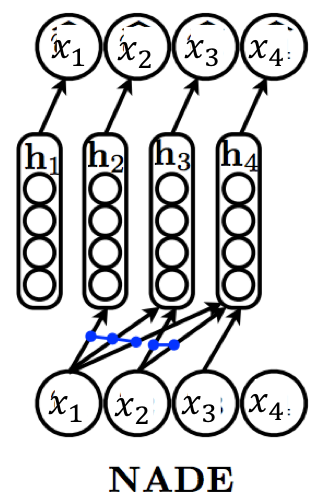
\includegraphics[scale=0.618]{pix/dgm/nade.png}
\caption{A neural autoregressive density estimator over four variables. The conditionals 
are denoted by \(\widehat{x}_1, \widehat{x}_2, \widehat{x}_3, \widehat{x}_4\) 
respectively. The blue connections denote the tied weights \(W[., i]\) used for 
computing the hidden layer activations.}
%\label{fig:label}
\end{figure}

The {\em Neural Autoregressive Density Estimator} (
\href{http://proceedings.mlr.press/v15/larochelle11a/larochelle11a.pdf}{NADE}) provides 
an alternate MLP-based parameterization that is more statistically and computationally 
efficient than the vanilla approach. In NADE, parameters are shared across the functions 
used for evaluating the conditionals. In particular, the hidden layer activations are 
specified as
$$
\mathbf{h}_i = \sigma(W_{., <i} \mathbf{x_{<i}} + \mathbf{c})\\
f_i(x_1, x_2, \ldots, x_{i-1}) =\sigma(\boldsymbol{\alpha}^{(i)}\mathbf{h}_i +b_i )  
$$
where $\theta=\{W\in \mathbb{R}^{d\times n}, \mathbf{c} \in \mathbb{R}^d, \{\boldsymbol{
\alpha}^{(i)}\in \mathbb{R}^d\}^n_{i=1}, \{b_i \in \mathbb{R}\}^n_{i=1}\}$ is the full set 
of parameters for the mean functions $f_1(\cdot), f_2(\cdot), \ldots, f_n(\cdot)$. The 
weight matrix $W$ and the bias vector $\mathbf{c}$ are shared across the conditionals. 
Sharing parameters offers two benefits:
\begin{enumerate}
\item[1.] 
The total number of parameters from $O(n^2 d)$ to $O(nd)$ [readers are encouraged 
to check!].

\item[2.] 
The hidden unit activations can be evaluated in $O(nd)$ time via the following 
recursive strategy:
$$
\mathbf{h}_i = \sigma(\mathbf{a}_i)\\
\mathbf{a}_{i+1} = \mathbf{a}_{i} + W[\cdot, i]x_i
$$
with the base case given by $\mathbf{a}_1=\mathbf{c}$.
\end{enumerate}


\subsubsection{Extensions to NADE}

The \href{https://arxiv.org/abs/1306.0186}{RNADE} algorithm extends NADE to learn 
generative models over real-valued data. Here, the conditionals are modeled via a 
continuous distribution such as a equi-weighted mixture of $K$ Gaussians. Instead 
of learning a mean function, we now learn the means $\mu_{i,1}, \mu_{i,2},\ldots, 
\mu_{i,K}$ and variances $\Sigma_{i,1}, \Sigma_{i,2},\ldots, \Sigma_{i,K}$ of the 
$K$ Gaussians for every conditional. For statistical and computational efficiency, 
a single function $g_i: \mathbb{R}^{i-1}\rightarrow\mathbb{R}^{2K}$ outputs all 
the means and variances of the $K$ Gaussians for the $i$-th conditional distribution.

Notice that NADE requires specifying a single, fixed ordering of the variables. The 
choice of ordering can lead to different models. 
The \href{https://arxiv.org/abs/1310.1757}{EoNADE} algorithm allows training an 
ensemble of NADE models with different orderings.


%+++++++++++++++++++++++++++++++++++++++++++
\subsection{Learning and inference}

Recall that learning a generative model involves optimizing the closeness between the 
data and model distributions. One commonly used notion of closeness in the KL 
divergence between the data and the model distributions.
\begin{align*}
\min_{\theta\in \mathcal{M}}d_{KL}
(p_{\mathrm{data}}, p_{\theta}) = \mathbb{E}_{\mathbf{x} \sim p_{\mathrm{data}} }
\left[\log p_{\mathrm{data}}(\mathbf{x}) - \log p_{\theta}(\mathbf{x})\right]
\end{align}

Before moving any further, we make two comments about the KL divergence. First, we note 
that the KL divergence between any two distributions is asymmetric. As we navigate through 
this chapter, the reader is encouraged to think what could go wrong if we decided to 
optimize the reverse KL divergence instead\footnote{这里是用 $p_\theta$ 的采样去逼近 
$p_{\mathrm{data}}$的分布,the reverse KL divergence 则是用 $p_{\mathrm{data}}$ 的采样去逼近 
$p_\theta$ 的分布}. Secondly, the KL divergences heavily penalizes 
any model distribution $p_\theta$ which assigns low probability to a datapoint that is 
likely to be sampled under $p_{\mathrm{data}}$. In the extreme case, if the density 
$p_\theta(\mathbf{x})$ evaluates to zero for a datapoint sampled from $p_{\mathrm{data}}$, 
the objective evaluates to $+\infty$.

Since $p_{\mathrm{data}}$ does not depend on $\theta$, we can equivalently recover the 
optimal parameters via maximizing likelihood estimation.
\begin{align*}
\max_{\theta\in \mathcal{M}}\mathbb{E}_{\mathbf{x} \sim p_{\mathrm{data}} }
\left[\log p_{\theta}(\mathbf{x})\right].
\end{align*}
Here, $\log p_{\theta}(\mathbf{x})$ is referred to as the log-likelihood of the datapoint 
$\mathbf{x}$ with respect to the model distribution $p_\theta$.

To approximate the expectation over the unknown $p_{\mathrm{data}}$, we make an assumption: 
points in the dataset $\mathcal{D}$ are sampled i.i.d\footnote{独立同分布,
independent and identically distributed}. from $p_{\mathrm{data}}$. This 
allows us to obtain an unbiased Monte Carlo estimate of the objective as
\begin{align}
\label{eq:mle}
\max_{\theta\in \mathcal{M}}\frac{1}{\vert D \vert} 
\sum_{\mathbf{x} \in\mathcal{D} }\log p_{\theta}(\mathbf{x}) 
= \mathcal{L}(\theta \vert \mathcal{D}).
\end{align}

The maximum likelihood estimation (MLE) objective has an intuitive interpretation: pick 
the model parameters $\theta \in \mathcal{M}$ that maximize the log-probability of the 
observed datapoints in $\mathcal{D}$.

In practice, we optimize the MLE objective using mini-batch gradient ascent. The algorithm 
operates in iterations. At every iteration $t$, we sample a mini-batch $\mathcal{B}_t$ 
of datapoints sampled randomly from the dataset ($\vert \mathcal{B}_t\vert < \vert 
\mathcal{D} \vert$) and compute gradients of the objective evaluated for the mini-batch. 
These parameters at iteration $t+1$ are then given via the following update rule
$$
\theta^{(t+1)} = \theta^{(t)} + r_t \nabla_\theta\mathcal{L}(\theta^{(t)} \vert 
\mathcal{B}_t)
$$
where $\theta^{(t+1)}$ and $\theta^{(t)}$ are the parameters at iterations $t+1$ and $t$ 
respectively, and $r_t$ is the learning rate at iteration $t$. Typically, we only specify 
the initial learning rate $r_1$ and update the rate based on a schedule. 
\href{http://cs231n.github.io/optimization-1/}{Variants} of stochastic gradient ascent, 
such as RMS prop and Adam, employ modified update rules that work slightly better in 
practice.

From a practical standpoint, we must think about how to choose hyperparameters (such as 
the initial learning rate) and a stopping criteria for the gradient descent. For both 
these questions, we follow the standard practice in machine learning of monitoring the 
objective on a validation dataset. Consequently, we choose the hyperparameters with the 
best performance on the validation dataset and stop updating the parameters when the 
validation log-likelihoods cease to improve\footnote{Given the non-convex nature of such 
problems, the optimization procedure can get stuck in local optima. Hence, early 
stopping will generally not be optimal but is a very practical strategy.}.

Now that we have a well-defined objective and optimization procedure, the only remaining 
task is to evaluate the objective in the context of an autoregressive generative model. 
To this end, we substitute the factorized joint distribution in 
Eq.$~\ref{eq:chain_rule}$ of an autoregressive model 
in the MLE objective in Eq.$~\ref{eq:mle}$ to get
$$
\max_{\theta \in \mathcal{M}}\frac{1}{\vert D \vert} \sum_{\mathbf{x} \in\mathcal{D} }
\sum_{i=1}^n\log p_{\theta_i}(x_i \vert \mathbf{x}_{< i})
$$
where $\theta = \{\theta_1, \theta_2, \ldots, \theta_n\}$ now denotes the
collective set of parameters for the conditionals.

Inference in an autoregressive model is straightforward. For density estimation of an 
arbitrary point $\mathbf{x}$, we simply evaluate the log-conditionals 
$\log p_{\theta_i}(x_i \vert \mathbf{x}_{< i})$ for each $i$ and add these up to obtain 
the log-likelihood assigned by the model to $\mathbf{x}$. Since we know conditioning 
vector $\mathbf{x}$, each of the conditionals can be evaluated in parallel. Hence, density 
estimation is efficient on modern hardware.

Sampling from an autoregressive model is a sequential procedure. Here, we first sample 
$x_1$, then we sample $x_2$ conditioned on the sampled $x_1$, followed by $x_3$ 
conditioned on both $x_1$ and $x_2$ and so on until we sample $x_n$ conditioned on the 
previously sampled $\mathbf{x}_{< n}$. For applications requiring real-time generation 
of high-dimensional data such as audio synthesis, the sequential sampling can be an 
expensive process. Later in this chapter, we will discuss how parallel WaveNet, an 
autoregressive model sidesteps this expensive sampling process.

% TODO: add NADE samples figure

Finally, an autoregressive model does not directly learn unsupervised representations of 
the data. In the next few set of lectures, we will look at latent variable models (e.g., 
variational autoencoders) which explicitly learn latent representations of the data.

% TODO: Autoregressive generative models based on Autoencoders, RNNs, and CNNs.
% MADE, Char-RNN, Pixel-CNN, Wavenet

% Additional parameterizations
% ==============
% Coming soon: MADE, Char-RNN, Pixel-CNN, Wavenet -->



%+++++++++++++++++++++++++++++++++++++++++++
\section{Variational Auto-Encoder}
%-------------------------------------------
% https://www.jianshu.com/p/ffd493e10751
% https://ychai.uk/notes/2020/01/09/Generative/Variational-AutoEncoders/


\begin{itemize}
%\setlength{\itemsep}{0pt}
%\setlength{\parsep}{0pt}
\setlength{\parskip}{0pt}
\item[-]
PixelCNN define tractable density function with MLE:
$$
p(\theta) = \prod_{i=1}^n p_\theta(x_i | x_1, \cdots, x_{i-1})
$$

\item[-]
VAE define the intractable density function with latent $\bz$:
$$
p(\theta) = \textcolor{red}{\int p_\theta(z) p_\theta(x|z) dz}
$$
\end{itemize}
This cannot directly optimize, VAEs derive and optimize the {\em lower bound} 
on likelihood instead.


%+++++++++++++++++++++++++++++++++++++++++++
\subsection{Auto-Encoder}

在说 VAE 之前,先来看一下它的前身 Auto-Encoder (AE)。AE 的初衷是为了数据降维。假设原始特征 $x$ 
维度过高,我们希望通过编码器 $E$ 将其编码成低维特征向量 $z=E(x)$,编码的原则是尽可能保留原始信息。
因此我们再训练一个解码器 $D$,希望能通过 $z$ 重构原始信息,即 $x\approx D(E(x))$,其优化目标一般是
$$
E,D = \argmin_{E,D}\mathbb{E}_{x\sim \D}\left[\|x-D(E(x))\|^2\right]
$$
AE 通过自监督的训练方式,
能够从原始特征获得一个潜在的特征编码,实现了自动化的特征工程,并且达到了降维和泛化的目的。
它的网络结构很简单,有编码 $E$ 和解码 $D$ 两个部分组成:

\begin{figure}[H]
\centering
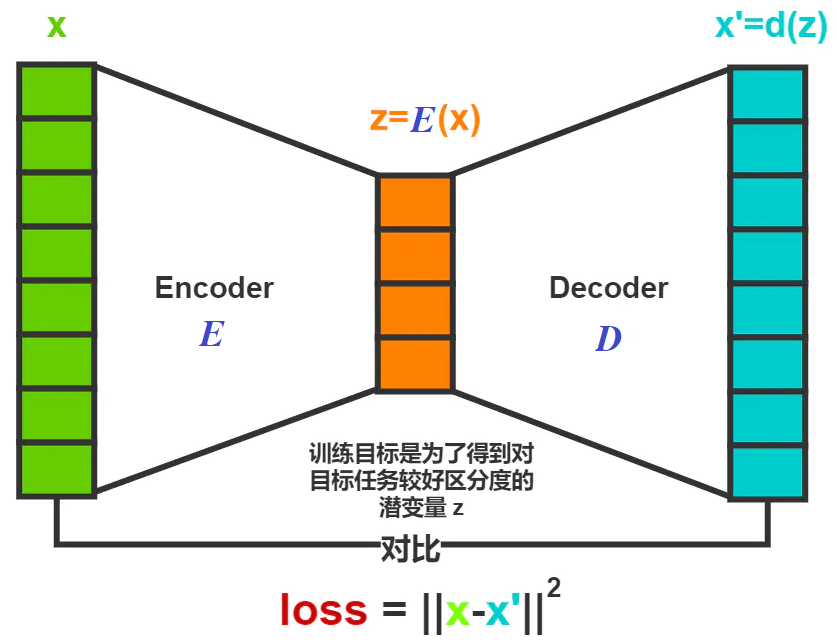
\includegraphics[scale=0.3]{pix/dgm/encoder_decoder.png}
\caption{Auto-Encoder}
%\label{fig:label}
\end{figure}

Autoencoder (AE) encodes the inputs into latent representations $\bz$ with dimension reduction 
to capture meaningful factors of variation in data. Then employ $\bz$ to reconstruct original 
data by autoencoding itself.

\begin{figure}[H]
\centering
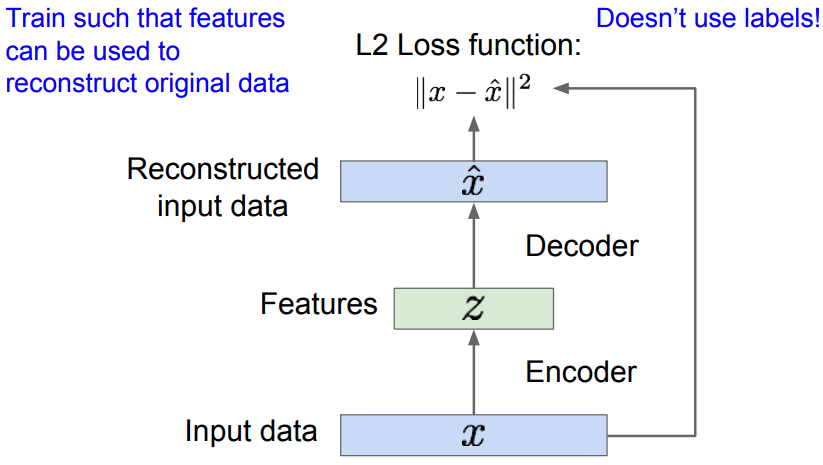
\includegraphics[scale=0.3]{pix/dgm/Autoencoder.png}
%\caption{Auto-Encoder}
%\label{fig:label}
\end{figure}

\begin{itemize}
%\setlength{\itemsep}{0pt}
%\setlength{\parsep}{0pt}
\setlength{\parskip}{0pt}
\item[-]
After training, throw away the decoder and {\bf only retain the encoder}.

\item[-]
Encoder can be used to initialize the supervised model on downstream tasks.
\end{itemize}

训练过程中加上一些扰动,就可以变成去噪自编码器(DAE):

\begin{figure}[H]
\centering
\includegraphics[scale=0.3]{pix/dgm/dae.png}
%\caption{Auto-Encoder}
%\label{fig:label}
\end{figure}

或者用遮盖(MIM,mask image modeling)的方法来加扰动

\begin{figure}[H]
\centering
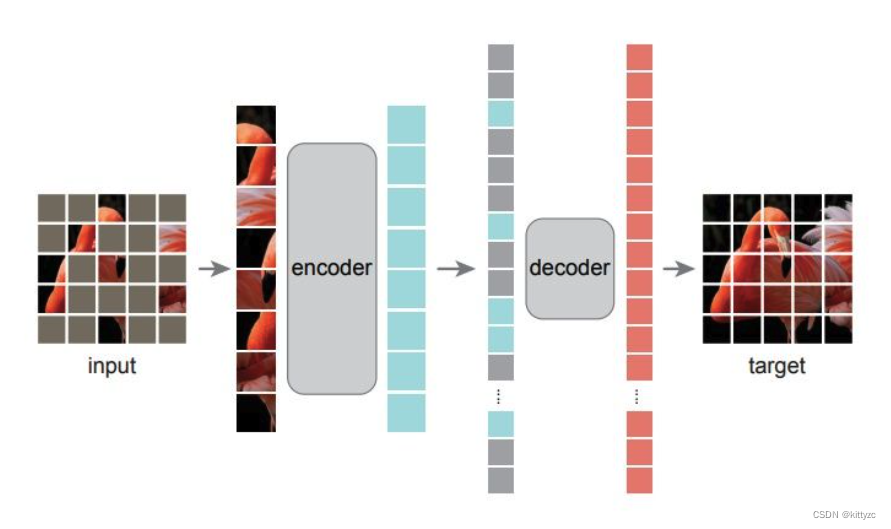
\includegraphics[scale=0.3]{pix/dgm/MIM.png}
%\caption{Auto-Encoder}
%\label{fig:label}
\end{figure}

容易看出,之所以是自监督就是因为网络的 target 即是 input 本身,因此不需要额外的标签工作,
虽然它由编码器和解码器两个部分组成,但是,显然从自编码器这个名字就可以看出,AE 的重点在于编码,
即得到这个隐藏层的向量,作为 input 的潜在特征,这是常见的一种 embedding 的一种方式。
而解码的结果,基于训练目标,如果损失足够小的话,将会与 input 相同,从这一点上看解码的值没有任何实际意义,
除了通过增加误差来补充平滑一些初始的零值或有些许用处。因为,从输入到输出的整个过程,
都是基于已有的训练数据的映射,尽管隐藏层的维度通常比输入层小很多,
但隐藏层的概率分布依然只取决于训练数据的分布,这就导致隐藏状态空间的分布并不是连续的,
于是如果我们随机生成隐藏层的状态,那么它经过解码将很可能不再具备输入特征的特点,
因此想通过解码器来生成数据就有点强模型所难了。


%+++++++++++++++++++++++++++++++++++++++++++
\subsection{VAE}

正是因为上面讨论过的那些原因,我们就需要对 AE 的隐藏层做些适当的改动,并进而形成所谓的 VAE。

\begin{figure}[H]
\centering
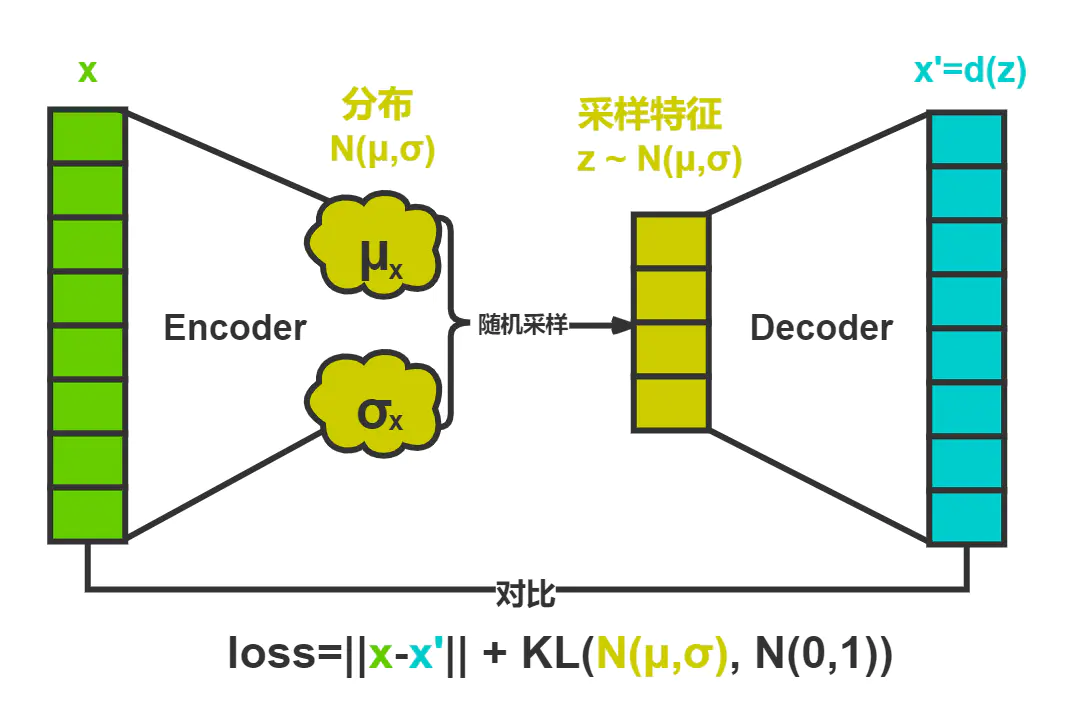
\includegraphics[scale=0.3]{pix/dgm/variational_encoder_decoder.png}
\caption{Variational Auto-Encoder}
%\label{fig:label}
\end{figure}

VAE 将输入和输出均看作是某个隐含变量 $\bz$(latent variable)的观测结果,输入和输出都是观测变量(observed 
variable)的采样结果,二者相对于对隐含变量都服从 Gaussian Distribution,都被看成是从这个分布进行采样的结果。
这样输入是一个采样,输出则是该采样通过神经网络解码的结果,目标函数是期望得到与输入相同的结果,损失函数几乎和 AE 一样,
只是增加编码推断分布与标准高斯分布的 KL 散度的正则项。增加这个正则项的目的是防止模型退化成普通的 AE,
这是因为网络优化过程中为了尽量减小重构误差,在训练过程中必然迫使方差逐渐被降到 0。
从而会逐渐丧失采样的随机性,进而最终退化成普通的 AE。

这里的重点是{\bf 采样}。其妙处是对每个输入 $\bx$, 对应一个概率分布 $p(\bx|\bz)$, 然后再从此分布中进行随机采样,
从而得到了连续完整的潜在空间,解决了 AE 中无法用于生成的问题。
这里的关键是把原始输入 $\bx$ 看作是一个表面观察特征(observed variable),而其对应的隐含特征(latent 
variable)$\bz$ 是一种深层抽象,其比观察特征更具备区分能力。在下一子节\ref{subsection_vae_representation}中,
我们将详细从理论上分析这种表示(representation)的细节。

\begin{figure}[H]
\centering
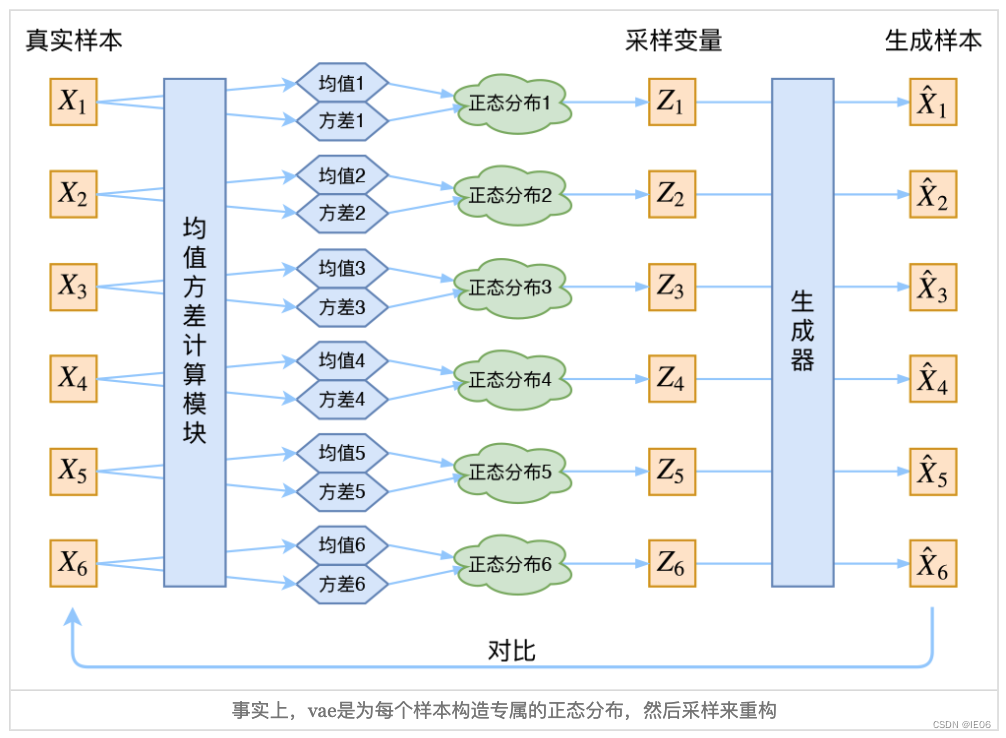
\includegraphics[scale=0.3]{pix/dgm/vae_details.png}
%\caption{Variational Auto-Encoder}
%\label{fig:label}
\end{figure}
上面我们已经谈到 VAE 的损失为重构误差 + KL散度。深入来看,对于每一个样本,需要用神经网络拟合均值 $u$ 
和方差 $\delta^2$,然后用标准正态分布采样得到 $\bz$,然后再恢复成 
$\bx$。其中方差项是核心,是用来进行对抗生成的关键。重构部分误差项会让 $u$ 尽量接近真实值,而 KL 
散度会保证生成器拥有标准的随机性。在后续的讨论中我们将称 $\bz$ 为隐含变量(latent variable), 而称 $\bx$ 
为观测变量(observed variable)。

Latent variable models form a rich class of probabilistic models that can infer hidden 
structure in the underlying data. In this section, we will study variational autoencoders, 
which are a powerful class of deep generative models with latent variables.


%+++++++++++++++++++++++++++++++++++++++++++
\subsection{Representation}
\label{subsection_vae_representation}

Consider a directed, latent variable model as shown below.

\begin{figure}[H]
\centering
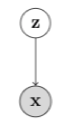
\includegraphics[scale=0.618]{pix/dgm/vae.png}
\caption{Graphical model for a directed, latent variable model.}
%\label{fig:label}
\end{figure}
\noindent
In the model above, $\bz$ and $\bx$ denote the latent and observed variables 
respectively. The joint distribution expressed by this model is given as
$$
p_\theta(\bx, \bz) = p(\bx \giv \bz)p(\bz).
$$

\begin{emp_box}\noindent
这里及后续要谈到的 representation 在数学上其实是最 cannonical 的表示,数学上有各种不同种类的表示,
例如小波框架表示甚至都不是正交表示(其基非正交,意味着表示也非唯一)。
显而易见的是这里的随机表示不是最恰当的数学表示方法。人类经常用类比来表达表示的方法,
AI 的算法似乎应该借鉴人类的表示方式,采样更妥当的表示方法来更贴近人类大脑的处理方式。
除了概率统计的方法,代数的方法、分析的方法都可以尝试一下。
\end{emp_box}

From a generative modeling perspective, this model describes a generative process for 
the observed data $\bx$ using the following procedure
\begin{align*}
\bz &\sim p(\bz) \\
\bx &\sim p(\bx \giv \bz).
\end{align}

If one adopts the belief that the latent variables $\bz$ somehow encode semantically 
meaningful information about $\bx$, it is natural to view this generative process as 
first generating the "high-level" semantic information about $\bx$ first before fully 
generating $\bx$. Such a perspective motivates 
\begin{itemize}
%\setlength{\itemsep}{0pt}
%\setlength{\parsep}{0pt}
\setlength{\parskip}{0pt}
\item[(1)]
generative models with rich latent 
variable structures such as hierarchical generative models $p(\bx, \bz_1, \ldots, \bz_m) 
= p(\bx \giv \bz_1)\prod_i p(\bz_i \giv \bz_{i+1})$ -- where information about $\bx$ 
is generated hierarchically, and 
\item[(2)]
temporal models such as the Hidden Markov Model -- where 
temporally-related high-level information is generated first before constructing $\bx$.
\end{itemize}

We now consider a family of distributions $\mathcal{P}_\bz$ where $p(\bz) \in \mathcal{P}_\bz$ describes 
a probability distribution over $\bz$. Next, consider a family of conditional 
distributions $\mathcal{P}_{\bx\giv \bz}$ where $p_\theta(\bx \giv \bz) \in \mathcal{P}_{\bx\giv \bz}$ 
describes a conditional probability distribution over $\bx$ given $\bz$. Then our 
hypothesis class of generative models is the set of all possible combinations
\begin{align*}
\mathcal{P}_{\bx,\bz} = \set{p(\bx, \bz) \giv p(\bz) \in \mathcal{P}_\bz, p(\bx \giv \bz) \in 
\mathcal{P}_{\bx\giv\bz}}.
\end{align}

Given a dataset $\D = \set{\bx^{(1)}, \ldots, \bx^{(n)}}$, we are interested in the 
following learning and inference tasks
\begin{itemize}
%\setlength{\itemsep}{0pt}
%\setlength{\parsep}{0pt}
\setlength{\parskip}{0pt}
\item[-]
Selecting $p \in \mathcal{P}_{\bx,\bz}$ that "best" fits $\D$.

\item[-]
Given a sample $\bx$ and a model $p \in \mathcal{P}_{\bx,\bz}$, what is the posterior 
distribution over the latent variables $\bz$?

\item[-]
Approximate marginal inference of $\bx$: given partial access to certain dimensions 
of the vector $\bx$, how do we impute the missing parts?
\end{itemize}

We shall also assume the following
\begin{itemize}
%\setlength{\itemsep}{0pt}
%\setlength{\parsep}{0pt}
\setlength{\parskip}{0pt}
\item[-]
Intractability: computing the posterior probability $p(\bz \giv \bx)$ is intractable.

\item[-]
Big data: the dataset $\D$ is too large to fit in memory; we can only work with 
small, sub-sampled batches of $\D$.
\end{itemize}

Representation (表示)的另一个说法是编码空间,不同的表示即选取不同的编码空间。
下面我们再从编码空间的角度看看 representation 的问题,或许能增强形象的理解。
{\bf 个人认为这里如果将编码空间叫做表示空间 (representation space) 似乎更恰当。}
\textcolor{blue}{从数据集 $\D$ 到表示空间 $\R$ 的映射可以看作是某种有限秩算子,这样前提是原始的算子必须是紧算子,
才可以用有限秩算子去逼近。文献中未见对该问题的仔细探究,我们有时间可以考虑一下该问题的恰当阐述方式。}

假如每个样本都可以重构得很好,那么我们可以将 $\bz$ 当作是 $\bx$ 
的等价表示,也就是说把 $\bz$ 研究好了就相当于把 $\bx$ 研究好了。现在我们将每个 $\bx$ 
都编码出对应的特征向量 $\bz$,然后我们关心一个问题:这些 $\bz$ 覆盖的空间的形态是个什么样子?

\begin{figure}[H]
\centering
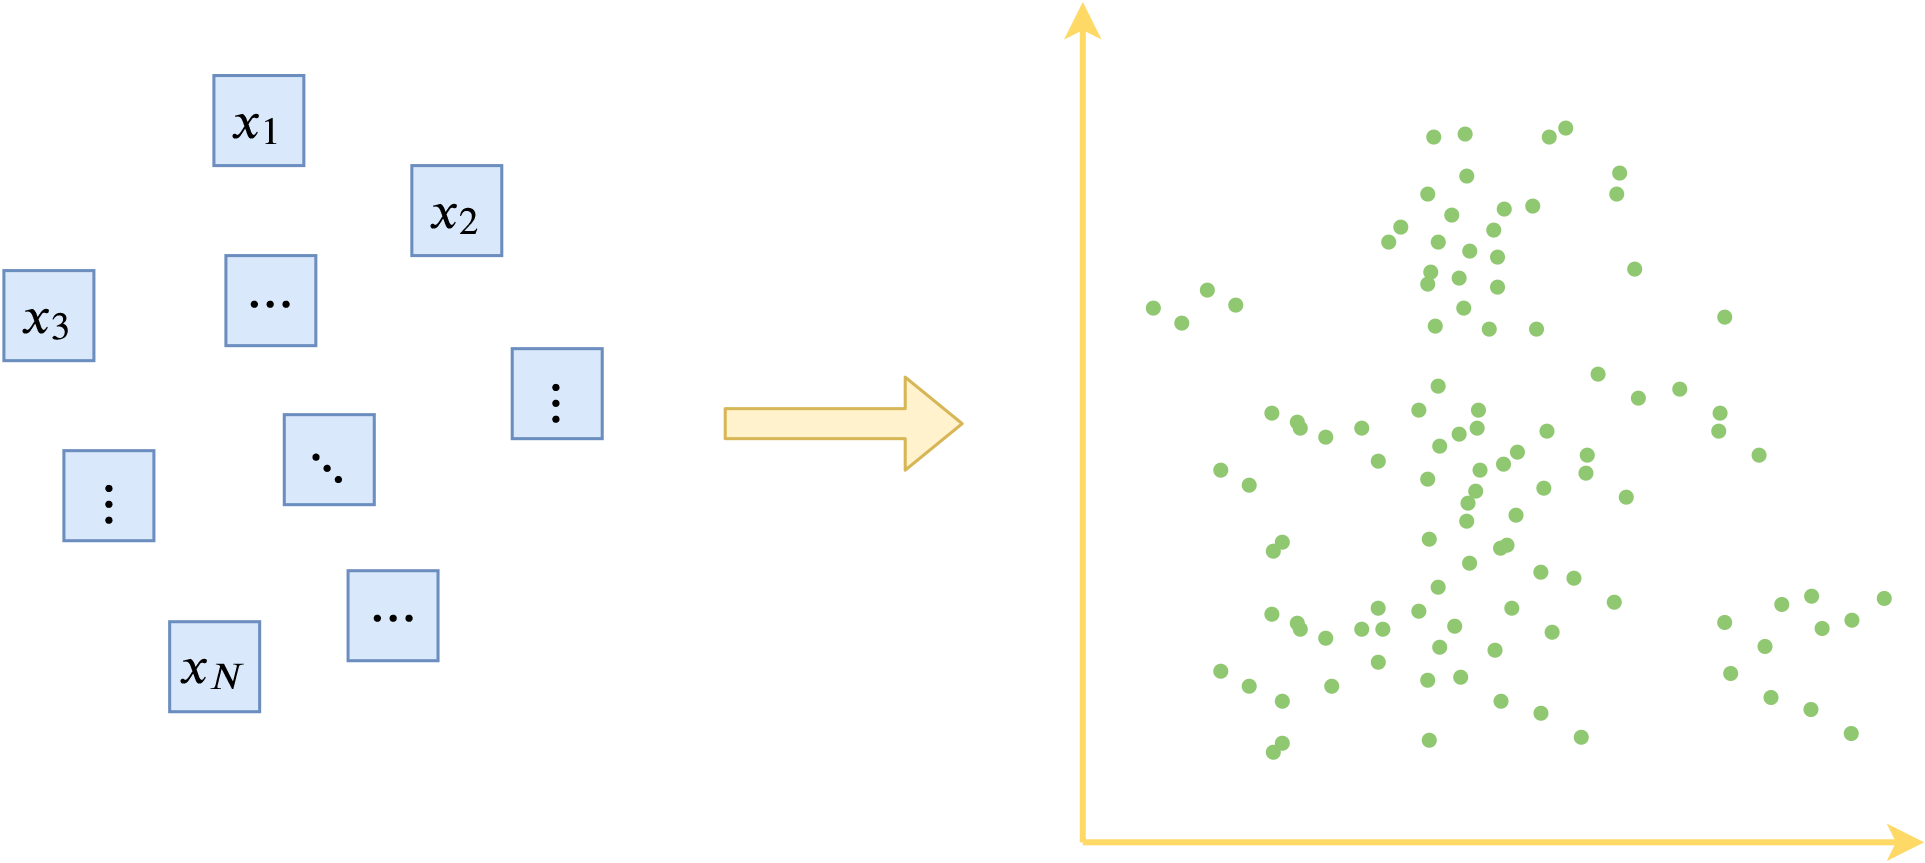
\includegraphics[scale=0.618]{pix/dgm/representation_space.png}
\caption{经过自编码器后,原始观测样本对应表示空间中的一个点}
%\label{fig:label}
\end{figure}

为什么要关心这个问题呢?因为我们可以有很多不同的编码表示方式,不同编码方式得到的特征向量也有好坏之分,
从“表示空间长什么样”可以大致地看出特征向量的好坏。比如下面四个不同的编码向量的分布形状模拟图:

\begin{figure}[H]
\centering
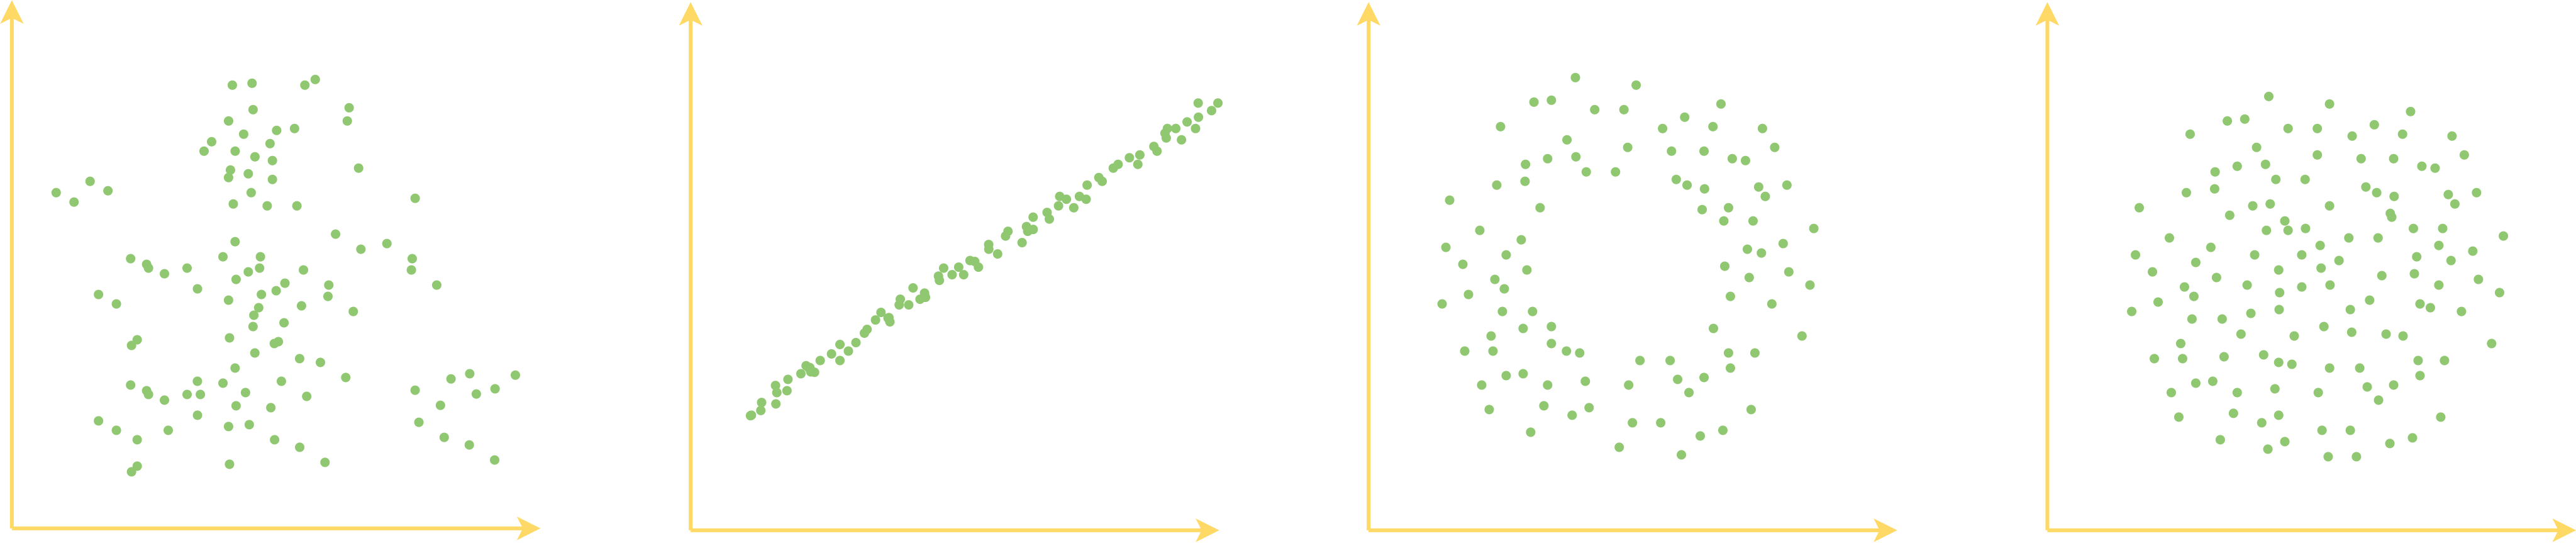
\includegraphics[scale=0.5]{pix/dgm/diff_represent_spaces.png}
\caption{四种不同的表示空间形状模拟图,分别代表无规律、线性、环形、圆形}
%\label{fig:label}
\end{figure}

第一个图的向量分布没什么特别的形状,比较散乱,说明编码空间并不是特别规整;第二个图的向量集中在一条线上,
说明其实编码向量的维度之间存在冗余;第三个图是一个环形,说明其圆心附近并没有对应的真实样本;第四个图是一个圆形,
表明它比较规整地覆盖了一块连续空间。就四个图来看,最后一个图所描绘的向量分布形状是最理想的:规整、无冗余、连续,
这意味着我们从中学习了一部分样本,就很容易泛化到未知的新样本上去,因为我们知道编码空间是规整连续的,
所以我们知道训练样本的编码向量之间的“缝隙”(图中的两个点之间的空白部分),实际上也对应着未知的真实样本,
因此把已知的搞好了,很可能未知的也搞好了。

\begin{emp_box}\noindent
研究思路:
\begin{itemize}
%\setlength{\itemsep}{0pt}
%\setlength{\parsep}{0pt}
\setlength{\parskip}{0pt}
\item[-]
多空间编码,区分不同特征

\item[-]
Mahananobis semi-normal 分布,消除相关性及重要性一致,偏置项的作用。

\item[-]
同胚映射,边界映射为边界。在目标函数中增加边界强化分离项。

\end{itemize}
\end{emp_box}

总的来说,大体上我们关心编码空间的如下问题:
\begin{itemize}
%\setlength{\itemsep}{0pt}
%\setlength{\parsep}{0pt}
\setlength{\parskip}{0pt}
\item[1.]
所有编码向量覆盖一个怎样的区域?

\item[2.]
是否有未知的真实样本对应空白之处的向量?

\item[3.]
有没有“脱离群众”的向量?

\item[4.]
有没有办法让编码空间更规整一些?
\end{itemize}

常规的自编码器由于没有特别的约束,因此很难回答上述问题。于是,变分自编码器出来了,从编码角度来看,它的目的是:
\begin{itemize}
%\setlength{\itemsep}{0pt}
%\setlength{\parsep}{0pt}
\setlength{\parskip}{0pt}
\item[1.]
让编码空间更规整一些;
\item[2.]
让编码向量更紧凑一些。
\end{itemize}
为了达到这个目的,变分自编码器先引入了后验分布 $p(z|x)$。

该怎么理解后验分布 $p(z|x)$ 呢?直观来看,我们可以将后验分布理解为一个“椭圆”,原来每个样本对应着一个编码向量,
也就是编码空间中的一个点,引入后验分布之后,相对于说现在每个样本 $x$ 都对应一个“椭圆”。刚才说希望编码向量更“紧凑”一些,
但理论上来讲,再多的“点”也没有办法把一个“面”覆盖完,但要是用“面”来覆盖“面”,那么就容易把目标覆盖住了。
这就是变分自编码器做出的主要改动之一。

\begin{figure}[H]
\centering
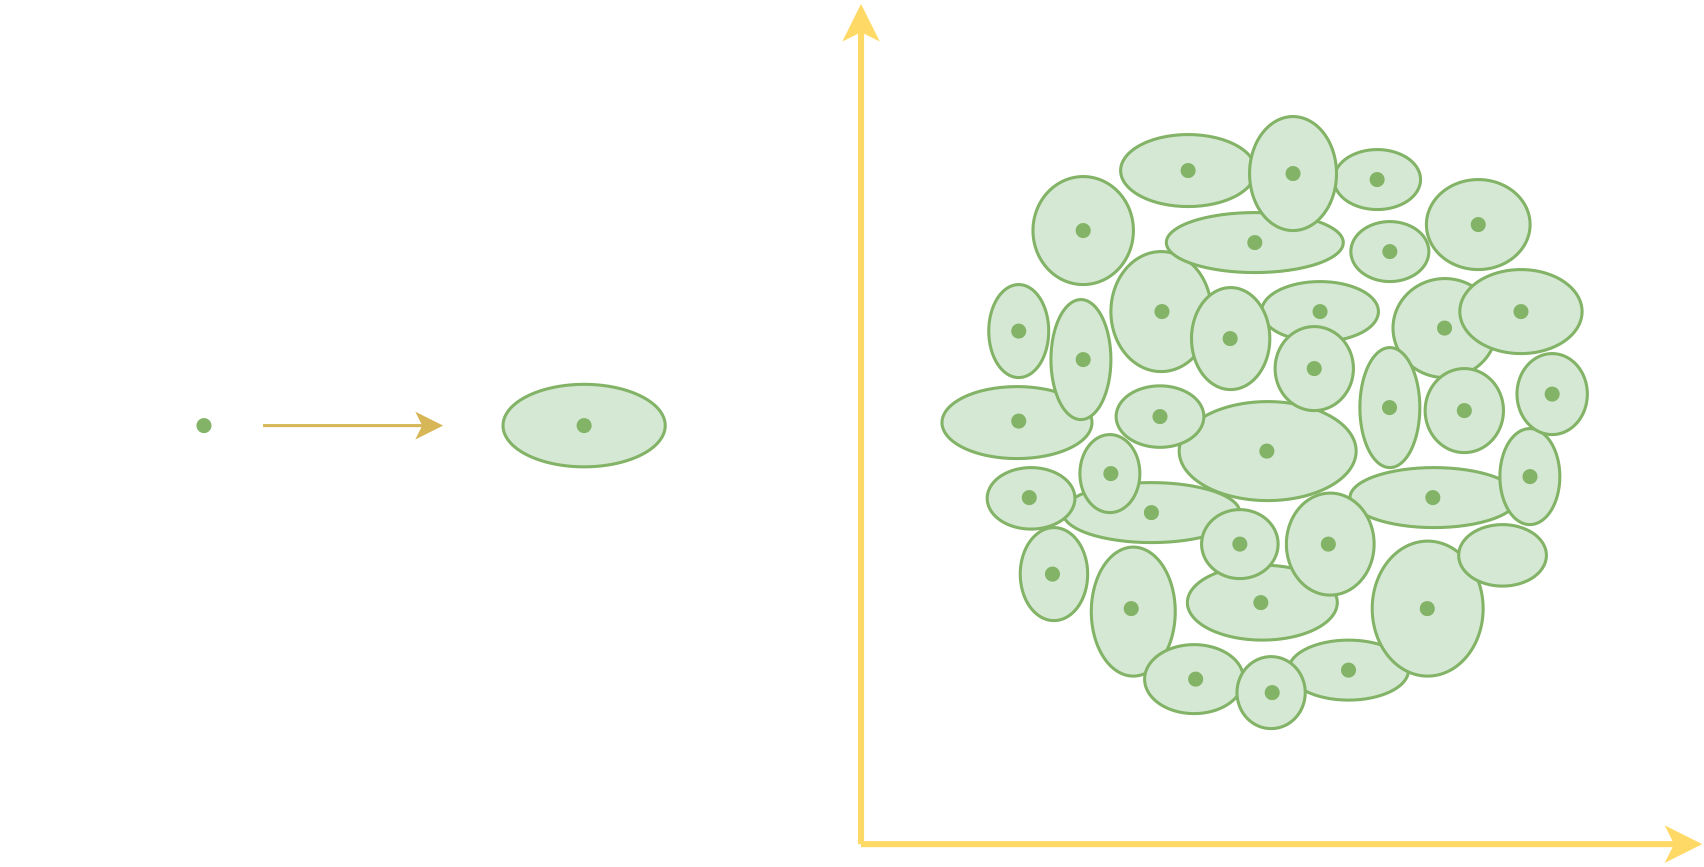
\includegraphics[scale=0.5]{pix/dgm/ellipse_cover.png}
\caption{每个样本的编码从一个点变成了一个面(椭圆),于是原本由点覆盖的编码空间变成了由面覆盖}
%\label{fig:label}
\end{figure}
为什么非得要椭圆呢?矩形或者其他形状可以吗?概率论中椭圆对应着“假设 $p(z|x)$ 各分量独立的高斯分布”,
从概率的角度来看,高斯分布是比较容易处理的一类概率分布,所以我们用高斯分布,也就对应着椭圆,
其他形状也就对应这其他分布,比如矩形可以跟均匀分布对应,但后面再算 KL 散度的时候会比较麻烦,因此一般不使用。


%+++++++++++++++++++++++++++++++++++++++++++
\subsection{采样重构与正则化}

现在每个样本 $x$ 都对应一个“椭圆”,而确定一个“椭圆”需要两个信息:椭圆中心、椭圆轴长,
它们各自构成一个向量,并且这个向量依赖于样本 $x$,我们将其记为 $\mu(x)$, $\sigma(x)$。
既然整个椭圆都对应着样本 $x$,我们要求椭圆内任意一点都可以重构 $x$,所以训练目标为:
$$
\mu, \sigma, D = \argmin_{\mu, \sigma, D} \mathbb{E}_{x\sim D} \left[ 
\| x - D(\mu(x) + \epsilon \otimes \sigma(x)) \|^2
\right], \quad \epsilon \sim \mathcal{N}(0, 1)
$$
其中 $D$ 是训练数据,$\mathcal{N}(0, 1)$ 为标准正态分布,我们可以将它理解为一个单位圆,
也就是说,我们先从单位圆内采样 $\epsilon$,然后通过平移缩放变换 $\mu(x) + \epsilon \otimes \sigma(x)$ 
将其变为“中心为 $\mu(x)$、轴长为 $\sigma(x)$”的椭圆内的点,这个过程就是所谓的“重参数(Reparameterization)”。

这里的 $\mu(x)$ 其实就对应于自编码器中的编码器 $E(x)$,$\sigma(x)$ 相当于它能泛化的范围。

正则化的过程本质上就是消除维度间冗余及各维度权重统一化的过程,典型的做法是 Mahananobis 
并加偏置来加强稳定性。

最终的变分自编码器:
\begin{align}
\mu, \sigma, D = \argmin_{\mu, \sigma, D} \mathbb{E}_{x\sim D} \left[ 
\| x - D(\mu(x) + \epsilon \otimes \sigma(x)) \|^2
+ \sum_{i=1}^d \frac{1}{2} \left(
\mu_i^2(x) + \sigma_i^2(x) - \log\sigma_i^2(x) - 1
\right) \right], \quad \epsilon \sim \mathcal{N}(0, 1)
\end{align}

%+++++++++++++++++++++++++++++++++++++++++++
\subsection{Learning Directed Latent Variable Models}

One way to measure how closely $p(\bx, \bz)$ fits the observed dataset $\D$ is to 
measure the Kullback-Leibler (KL) divergence between the data distribution (which 
we denote as $p_{\mathrm{data}}(\bx)$) and the model's marginal distribution 
$p(\bx) = \int p(\bx, \bz) \d \bz$. The distribution that ``best'' fits the data is 
thus obtained by minimizing the KL divergence. 
\begin{align*}
\min_{p \in \P_{\bx, \bz}}\KL{p_{\mathrm{data}}(\bx)}{p(\bx)}.
\end{align}

As we have seen previously, optimizing an empirical estimate of the KL divergence is 
equivalent to maximizing the marginal log-likelihood $\log p(\bx)$ over $\D$
\begin{align*}
\max_{p \in \P_{\bx, \bz}} \sum_{\bx \in \D} \log p(\bx) = \sum_{\bx \in \D} \log\int p(\bx, \bz) \d \bz.
\end{align}

However, it turns out this problem is generally intractable for high-dimensional $\bz$ 
as it involves an integration (or sums in the case $\bz$ is discrete) over all the 
possible latent sources of variation $\bz$. One option is to estimate the objective 
via Monte Carlo. For any given datapoint $\bf x$, we can obtain the following estimate 
for its marginal log-likelihood
$$
\log p(\bx) \approx \log \frac{1}{k} \sum_{i=1}^k p(\bx \vert \bz^{(i)}) \text{, where } \bz^{(i)} \sim p(\bz)
$$

In practice however, optimizing the above estimate suffers from high variance in 
gradient estimates. 

Rather than maximizing the log-likelihood directly, an alternate is to instead 
construct a lower bound that is more amenable to optimization. To do so, we note that 
evaluating the marginal likelihood $p(\bx)$ is at least as difficult as as evaluating 
the posterior $p(\bz \mid \bx)$ for any latent vector $\bz$ since by definition 
$p(\bz \mid \bx) = p(\bx, \bz) / p(\bx)$. 

\begin{emp_box}\noindent
By now it seems that $p(\bz \mid \bx)$ and $p(\bx \mid \bz)$ are dual distributions, 
$\P$ and $\Q$ are dual spaces. Can we employ Galerkin method to do all the analysis?
更进一步,在非 VAE 的场景,似乎也有相应的问题,这里不过正好是自监督。非自监督的场景将是真正的对偶,
测试空间与算子空间形成对偶。
\end{emp_box}

Next, we introduce a variational family $\Q$ of distributions that approximate the 
true, but intractable posterior $p(\bz \mid \bx)$. Further henceforth, we will assume 
a parameteric setting where any distribution in the model family $\P_{\bx, \bz}$ is 
specified via a set of parameters $\theta \in \Theta$ and distributions in the 
variational family $\Q$ are specified via a set of parameters $\lambda \in \Lambda$. 

Given $\P_{\bx, \bz}$ and $\Q$, we note that the following relationships hold 
true\footnote{The first equality only holds if the support of $q$ includes that of 
$p$. If not, it is an inequality.} for any $\bx$ and all variational distributions 
$q_\lambda(\bz) \in \Q$
\begin{align*}
\log p_\theta(\bx) &= \log \int p_\theta(\bx, \bz) \d \bz \\
&= \log \int \frac{q_\lambda(\bz)}{q_\lambda(\bz)} p(\bx, \bz) \d \bz\\
&\ge\int q_\lambda(\bz) \log \frac{p_\theta(\bx, \bz)}{q_\lambda(\bz)} \d \bz \\
&= \Expect_{q_\lambda(\bz)} \left[\log \frac{p_\theta(\bx, \bz)}{q_\lambda(\bz)}\right] \\
&:=\ELBO(\bx; \theta, \lambda)
\end{align}
where we have used Jensen's inequality in the final step. The Evidence Lower Bound 
or ELBO in short admits a tractable unbiased Monte Carlo estimator
\begin{align*}
\frac{1}{k} \sum_{i=1}^k \log \frac{p_\theta(\bx, \bz^{(i)})}{q_\lambda(\bz^{(i)})} \text{, where } \bz^{(i)} \sim q_\lambda(\bz),
\end{align}
so long as it is easy to sample from and evaluate densities for $q_\lambda(\bz)$. 

Which variational distribution should we pick? Even though the above derivation holds 
for any choice of variational parameters $\lambda$, the tightness of the lower bound 
depends on the specific choice of $q$. 

\begin{figure}[H]
\centering
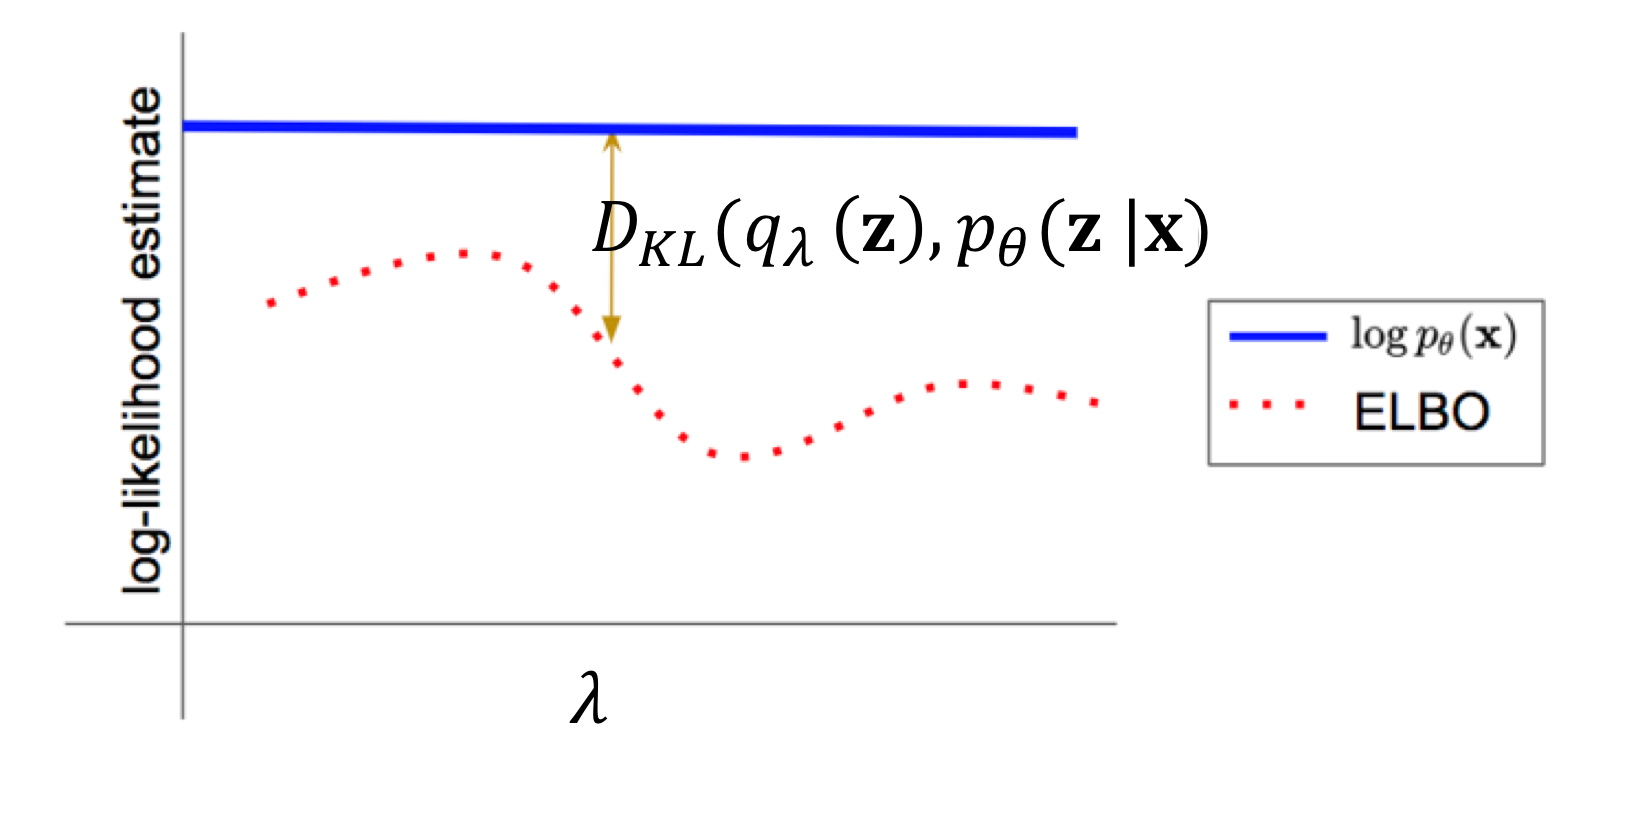
\includegraphics[scale=0.318]{pix/dgm/klgap.png}
\caption{Illustration for the KL divergence gap between the marginal log-likelihood 
\(\log p_\theta(\bx)\) for a point \(\bx\) and the corresponding ELBO for a 
single 1D-parameter variational distribution \(q_\lambda(\bx)\).}
%\label{fig:label}
\end{figure}

In particular, the gap between the original objective(marginal log-likelihood 
$\log p_\theta(\bx) $) and the ELBO equals the KL divergence between the approximate 
posterior $q(\bz)$ and the true posterior $p(\bz \giv \bx)$. The gap is zero when the 
variational distribution $q_\lambda(\bz)$ exactly matches $p_\theta(\bz \giv \bx)$. 

In summary, we can learn a latent variable model by maximizing the ELBO with respect 
to both the model parameters $\theta$ and the variational parameters $\lambda$ for any 
given datapoint $\bx$

\begin{align}
\max_{\theta} \sum_{\bx \in \D} \max_{\lambda} \Expect_{q_\lambda(\bz)} \left[\log \frac{p_\theta(\bx, \bz)}{q_\lambda(\bz)}\right].
\end{align}


%+++++++++++++++++++++++++++++++++++++++++++
\subsection{Black-Box Variational Inference}

In this subsection, we shall focus on first-order stochastic gradient methods for 
optimizing the ELBO. These optimization techniques are desirable in that they allow 
us to sub-sample the dataset during optimization---but require our objective function 
to be differentiable with respect to the optimization variables. 

As such, we shall posit for now that any $p(\bx, \bz) \in \P_{\bx, \bz}$ and 
$q(\bz) \in \Q$ are alternatively parameterizable as $p_\theta(\bx, \bz)$ and 
$q_\lambda(\bz)$ and that these distributions are differentiable with respect to 
$\theta$ and $\lambda$.

This inspires Black-Box Variational Inference (BBVI), a general-purpose 
Expectation-Maximization-like algorithm for variational learning of latent variable 
models, where, for each mini-batch $\M = \set{\bx^{(1)}, \ldots, \bx^{(m)}}$, the 
following two steps are performed.


\subsubsection{Step 1}

We first do {\bf per-sample} optimization of $q$ by iteratively applying the update
\begin{align}
\lambda^{(i)} \gets \lambda^{(i)} + \tilde{\nabla}_\lambda \ELBO(\bx^{(i)}; \theta, \lambda^{(i)}),
\end{align}
where $\text{ELBO}(\bx; \theta, \lambda) 
= \Expect_{q_\lambda(\bz)} \left[\log \frac{p_\theta(\bx, \bz)}{q_\lambda(\bz)}\right]$, and 
$\tilde{\nabla}_\lambda$ denotes an unbiased estimate of the ELBO gradient. This step seeks to 
approximate the log-likelihood $\log p_\theta(\bx^{(i)})$.

\subsubsection{Step 2}

We then perform a single update step based on the mini-batch
\begin{align}
\theta \gets \theta + \tilde{\nabla}_\theta \sum_{i} \ELBO(\bx^{(i)}; \theta, \lambda^{(i)}),
\end{align}
which corresponds to the step that hopefully moves $p_\theta$ closer to $p_{\mathrm{data}}$.


%+++++++++++++++++++++++++++++++++++++++++++
\subsection{Gradient Estimation}

The gradients $\nabla_\lambda \ELBO$ and $\nabla_\theta \ELBO$ can be estimated via Monte Carlo 
sampling. While it is straightforward to construct an unbiased estimate of $\nabla_\theta \ELBO$ 
by simply pushing $\nabla_\theta$ through the expectation operator, the same cannot be said for 
$\nabla_\lambda$. Instead, we see that
\begin{align}
\nabla_\lambda \Expect_{q_\lambda(\bz)} \left[\log \frac{p_\theta(\bx, \bz)}{q_\lambda(\bz)} \right]= \Expect_{q_\lambda(\bz)} \brac{\paren{\log \frac{p_\theta(\bx, \bz)}{q_\lambda(\bz)}} \cdot \nabla_\lambda \log q_\lambda(\bz)}.
\end{align}
This equality follows from the log-derivative trick (also commonly referred to as the REINFORCE 
trick). The full derivation involves some simple algebraic manipulations and is left as an exercise 
for the reader. The gradient estimator $\tilde{\nabla}_\lambda \ELBO$ is thus
\begin{align}
\frac{1}{k}\sum_{i=1}^k \brac{\paren{\log \frac{p_\theta(\bx, \bz^{(i)})}{q_\lambda(\bz^{(i)})}} \cdot \nabla_\lambda \log q_\lambda(\bz^{(i)})} \text{, where } \bz^{(i)} \sim q_\lambda(\bz).
\end{align}
However, it is often noted that this estimator suffers from high variance. One of the key 
contributions of the variational autoencoder paper is the reparameterization trick, which introduces 
a fixed, auxiliary distribution $p(\veps)$ and a differentiable function $T(\veps; \lambda)$ such 
that the procedure
\begin{align}
\veps &\sim p(\veps)\\
\bz &\gets T(\veps; \lambda),
\end{align}
is equivalent to sampling from $q_\lambda(\bz)$. By the 
\href{https://en.wikipedia.org/wiki/Law_of_the_unconscious_statistician}{Law of the Unconscious Statistician}, 
we can see that
\begin{align}
\nabla_\lambda \Expect_{q_\lambda(\bz)} \left[\log \frac{p_\theta(\bx, \bz)}{q_\lambda(\bz)}\right] = \Expect_{p(\veps)} \left[\nabla_\lambda \log \frac{p_\theta(\bx, T(\veps; \lambda))}{q_\lambda(T(\veps; \lambda))}\right].
\end{align}
In contrast to the REINFORCE trick, the reparameterization trick is often noted empirically to have 
lower variance and thus results in more stable training. 

\rs{I think there exists pathological examples where REINFORCE has lower variance than reparamterization. 
Should we talk about that?}


%+++++++++++++++++++++++++++++++++++++++++++
\subsection{Parameterizing Distributions via Deep Neural Networks}

So far, we have described $p_\theta(\bx, \bz)$ and $q_\lambda(\bz)$ in the abstract. To 
instantiate these objects, we consider choices of parametric distributions for 
$p_\theta(\bz)$, $p_\theta(\bx \giv \bz)$, and $q_\lambda(\bz)$. A popular choice for 
$p_\theta(\bz)$ is the unit Gaussian
\begin{align}
p_\theta(\bz) = \Normal(\bz \giv \0, \I).
\end{align}
in which case $\theta$ is simply the empty set since the prior is a fixed distribution. 
Another alternative often used in practice is a mixture of Gaussians with trainable mean 
and covariance parameters. 

The conditional distribution $p_\theta(\bx \giv \bz)$ is where we introduce a deep neural 
network. We note that a conditional distribution can be constructed by defining a 
distribution family (parameterized by $\omega \in \Omega$) in the target space $\bx$ (i.e. 
$p_\omega(\bx)$ defines an unconditional distribution over $\bx$) and a mapping function 
$g_\theta: \Z \to \Omega$. 

It is natural to call $g_\theta$ the decoder that is parameterized by $\theta$. The act of 
conditioning on $\bz$ is thus equivalent to using the choice of $\omega = g(\bz)$. 

In other words, $g_\theta(\cdot)$ defines the conditional distribution
\begin{align}
    p_\theta(\bx \giv \bz) = p_\omega(\bx) \text{ , where } \omega = g_\theta(\bz).
\end{align}
The function $g_\theta$ is also referred to as the decoding distribution since it maps a 
latent {\em code} $\bz$ to the parameters of a distribution over observed variables $\bx$. 
In practice, it is typical to specify $g_\theta$ as a deep neural network.  

The generative model $p_\theta(\bx, \bz)$ is called a {\em deep} generative model since we 
will be using a neural network to instantiate the function $g_\theta$.

In the case where $p_\theta(\bx \giv \bz)$ is a Gaussian distribution, we can thus 
represent it as
\begin{align}
    p_\theta(\bx \giv \bz) = \Normal(\bx \giv \mu_\theta(\bz), \Sigma_\theta(\bz)),
\end{align}
where $\mu_\theta(\bz)$ and $\Sigma_\theta(\bz)$ are neural networks that specify the mean 
and covariance matrix for the Gaussian distribution over $\bx$ when conditioned on $\bz$.

Finally, the variational family for the proposal distribution $q_\lambda(\bz)$ needs to be 
chosen judiciously so that the reparameterization trick is possible. Many continuous 
distributions in the 
\href{https://en.wikipedia.org/wiki/Location%E2%80%93scale_family}{location-scale family} 
can be reparameterized. In practice, a popular choice is again the Gaussian distribution, 
where
\begin{align*}
    \lambda &= (\mu, \Sigma) \\
    q_\lambda(\bz) &= \Normal(\bz \giv \mu, \Sigma)\\
    p(\veps) &= \Normal(\veps \giv \0, \I) \\
    T(\veps; \lambda) &= \mu + \Sigma^{1/2}\veps,
\end{align}
where $\Sigma^{1/2}$ is the Cholesky decomposition of $\Sigma$. For simplicity, practitioners 
often restrict $\Sigma$ to be a diagonal matrix (which restricts the distribution family to 
that of factorized Gaussians).


%+++++++++++++++++++++++++++++++++++++++++++
\subsection{Amortized Variational Inference}

A noticeable limitation of black-box variational inference is that {\bf Step 1} executes an 
optimization subroutine that is computationally expensive. Recall that the goal of the {\bf 
Step 1} is to find
\begin{align}
    \lambda^* = \argmax_{\lambda\in \Lambda} \ELBO(\bx; \theta, \lambda).
\end{align}
For a given choice of $\theta$, there is a well-defined mapping from $\bx \mapsto \lambda^\ast$. 
A key realization is that this mapping can be {\em learned}. In particular, one can train an 
encoding function (parameterized by $\phi$) $f_\phi: \X \to \Lambda$ 
(where $\Lambda$ is the space of $\lambda$ parameters) 
on the following objective
\begin{align}
    \max_{\phi } \sum_{\bx \in \D} \ELBO(\bx; \theta, f_\phi(\bx)).
\end{align}
It is worth noting at this point that $f_\phi(\bx)$ can be interpreted as defining the 
conditional distribution $q_\phi(\bz \giv \bx)$. With a slight abuse of notation, we define
\begin{align}
    \ELBO(\bx; \theta, \phi) = \Expect_{q_\phi(\bz \mid \bx)} \left[\log \frac{p_\theta(\bx, \bz)}{q_\phi(\bz \giv \bx)}\right].
\end{align}
and rewrite the optimization problem as 
\begin{align}
    \max_{\phi } \sum_{\bx \in \D} \ELBO(\bx; \theta, \phi).
\end{align}
It is also worth noting that optimizing $\phi$ over the entire dataset as a {\em subroutine} 
every time we sample a new mini-batch is clearly not reasonable. However, if we believe that 
$f_\phi$ is capable of quickly adapting to a close-enough approximation of $\lambda^\ast$ 
given the current choice of $\theta$, then we can interleave the optimization $\phi$ and 
$\theta$. This yields the following procedure, where for each mini-batch 
$\M = \set{\bx^{(1)}, \ldots, \bx^{(m)}}$, we perform the following two updates jointly
\begin{align}
    \phi &\gets \phi + \tilde{\nabla}_\phi \sum_{\bx \in \M} \ELBO(\bx; \theta, \phi) \\
    \theta &\gets \theta + \tilde{\nabla}_\theta \sum_{\bx \in \M} \ELBO(\bx; \theta, \phi),
\end{align}
rather than running BBVI's {\bf Step 1} as a subroutine. By leveraging the learnability of 
$\bx \mapsto \lambda^\ast$, this optimization procedure amortizes the cost of variational 
inference. If one further chooses to define $f_\phi$ as a neural network, the result is the 
variational autoencoder.


%+++++++++++++++++++++++++++++++++++++++++++
\section{变分自编码是怎么炼成的}
%-------------------------------------------

读了上面的内容之后,你应该对 VAE 模型有了一个较为直观和感性的认知,但是可能会疑惑所谓的变分到底在哪里?
放心,变分并没有被作者吃掉,接下来,我们就从变分推断的角度,对 VAE 进行一个理性的推导。有了上面的基础,
再读下面的内容时就会轻松愉快很多。


%+++++++++++++++++++++++++++++++++++++++++++
\subsection{变分推断}

变分自编码器(VAE)的想法和名字的由来便是变分推断了,那么什么是变分推断呢?
变分推断是 MCMC 搞不定场景的一种替代算法,它考虑一个贝叶斯推断问题,给定观测变量 $x\in\mathbb{R}^n$ 
和潜变量 $z\in\mathbb{R}^d$, 其联合概率分布为 $p(z,x) = p(z)p(x|z)$, 目标是计算后验分布 
$p(z|x)$。然后我们可以假设一个变分分布 $q(z)$ 来自分布族 $Q$,通过最小化 KL 散度来近似后验分布 
$p(z|x)$:
$$
q^* = \operatorname{arg min}_{q(z)\in Q} D_{KL}(q(z) ~ \| ~ p(z|x))
$$
这么一来,就成功的将一个贝叶斯推断问题转化为了一个优化问题。


%+++++++++++++++++++++++++++++++++++++++++++
\subsection{变分推导过程}

有了变分推断的认知,我们再回过头去看一下 VAE 模型的整体框架。VAE 就是将 AE 
的编码和解码过程转化为了一个贝叶斯概率模型:我们的训练数据即为观测变量 $x$,
假设它由不能直接观测到的潜变量 $z$ 生成。于是,生成观测变量过程便是似然分布:$p(x | z)$,
也就是解码器,因而编码器自然就是后验分布:$p(z | x)$。根据贝叶斯公式,建立先验、后验和似然的关系:
$$
p(z|x) = \frac{p(x|z)p(z)}{p(x)} = \int_z\frac{p(x|z)p(z)}{p(x)}dz
$$
接下来,基于上面变分推断的思想,我们假设变分分布 $q_x(z)$, 通过最小化 KL 散度来近似后验分布 $p(z|x)$,
于是,最佳的 $q_x^*$ 便是:
\begin{align*}
q_x^* &= \operatorname{arg min}\left( D_{KL}(q_x(z) \| p(z|x)) \right) \\
&= \operatorname{arg min}\left( \mathbb{E}_{q_x(z)}\left[ 
\log q_x(z) - \log p(x|z) - \log p(z) \right] + \log p(x) \right)
\end{align}
因为训练数据 $x$ 是确定的,因此 $\log~p(x)$ 是一个常数,于是上面的优化问题等价于:
\begin{align*}
q_x^* &= \operatorname{arg min}\left( \mathbb{E}_{q_x(z)}\left[ 
\log q_x(z) - \log p(x|z) - \log p(z) \right] \right) \\
&= \operatorname{arg min}\left( \mathbb{E}_{q_x(z)}\left[ 
 - \log p(x|z) + (\log q_x(z) - \log p(z)) \right] \right) \\
&= \operatorname{arg min}\left( \mathbb{E}_{q_x(z)}\left[ 
 - \log p(x|z) + D_{KL}(q_x(z) ~\|~ p(z)) \right] \right)
\end{align}

此时,优观察一下优化方程的形式,已经是我们前面所说的 VAE 的损失函数了。
显然,跟我们希望解码准确的目标是一致的。要解码的准,则 $p(x|z)$ 应该尽可能的小,编码特征 $z$ 
的分布 $q_x(z)$ 同 $p(z)$ 尽可能的接近。此时恰好 $-\log p(x|z)$ 和 $D_{KL}(q_x(z) \| p(z|x))$ 
都尽可能的小,与损失的优化的目标也一致。


%+++++++++++++++++++++++++++++++++++++++++++
\subsection{如何计算极值}

正如前面所提到的 AE 潜变量的局限性,我们希望 VAE 的潜变量分布 $p(z)$ 应该能满足海量的输入数据 $x$ 
并且相互独立。基于中心极限定理,以及为了方便采样,我们有理由直接假设 $p(z)$ 是一个标准的高斯分布 
$\mathcal{N}(0,1)$。


\subsubsection{编码部分}

我们先来看一下编码部分,我们希望拟合一个分布 $q_x(z) = \mathcal{N}(\mu, \sigma)$ 尽可能接近 
$p(z) = \mathcal{N}(0,1)$。关键就在于基于输入 $x$ 计算 $\mu$ 和 $\sigma$。直接算有点困难,
于是就使用两个神经网络 $f(x)$ 和 $g(x)$ 来无脑拟合 $\mu$ 和 $\sigma$。

值得一提的是,很多地方实际使用的 $f(x)$、$g(x)$ 两部分神经网络并不是独立的,而是有一部分交集。
即他们都先通过一个 $h(x)$ 映射到一个中间层 $h$, 然后分别对 $h$ 计算 $f(h)$ 和 $g(h)$。
这样做的好处一方面是可以减少参数数量,另外也会导致拟合的效果差一些,算是防止过拟合吧。


\subsubsection{解码部分}

解码,即从潜变量 $z$ 生成数据 $x$ 的过程,在于最大化似然 $p(x|z)$,那这应该是个什么分布呢?
通常我们假设它是一个{\bf 伯努利分布}或是{\bf 高斯分布}。
这是因为伯努利分布简单,高斯分布自然。

知道了分布类型,那计算 $-\log p(x|z)$ 最小值其实只要把分布公式带进去算就可以了。

\begin{itemize}
%\setlength{\itemsep}{0pt}
%\setlength{\parsep}{0pt}
\setlength{\parskip}{0pt}
\item[-]
高斯分布
\begin{align*}
\operatorname{arg min}(-\log q(x|z))
&= \operatorname{arg min}\frac{1}{2}
\left\| \frac{x-\tilde{\mu}(z)}{\tilde{\sigma}(z)} \right\|^2 
+ \frac{c}{2}\log 2\pi + \frac{1}{2} \\
&= \operatorname{arg min}\frac{1}{2}
\left\| \frac{x-\tilde{\mu}(z)}{\tilde{\sigma}(z)} \right\|^2
\end{align}
和预期一样,演变为了均方误差。

\item[-]
伯努利分布
假设伯努利的二元分布是 $p$ 和 $1-p$ (注意这里是输出没一维组成的向量)
$$
\operatorname{arg min}(-\log q(x|z)) = \operatorname{arg min}(-x\log p - (1-x)\log(1-p))
$$
很对,正好就是交叉熵的损失。
\end{itemize}

然后,将编码和解码部分组合到一起,就形成了完整的 VAE 网络。



%+++++++++++++++++++++++++++++++++++++++++++
\subsection{一点微不足道的技巧}

训练的时候似乎出了点问题。从编码得到的分布 $\mathcal{N}(\mu,\sigma)$ 随机采样 $z$ 
的这个过程没法求导,没法进行误差反向传播。这里可以使用一个叫做重参数(reparametrisation trick) 的技巧:
$$
z=f(x)\zeta + g(x), \qquad \zeta\sim N(0,1)
$$
真是妙呀,这样一来将采样变成了一个数值变换,整个过程便可导了。

这样,训练好模型之后,我们可以直接将解码部分拿出来,通过标准高斯分布随机采样源源不断的生成数据了。

%+++++++++++++++++++++++++++++++++++++++++++
\subsection{延伸的一些思考}

VAE 中使用神经网络来拟合高斯分布的想法独树一帜,对很多任务能带来启发。
神经网络在特征化训练数据的过程无异于海量数据的管中窥豹,但是想要让模型超脱于豹,
而像人一样产生对相似的猫、老虎...之类的概念,VAE 的这种思想颇有一些意味。

\href{https://arxiv.org/pdf/1312.6114.pdf}{Auto-Encoding Variational Bayes}

\href{}{Understanding Variational Autoencoders}



%+++++++++++++++++++++++++++++++++++++++++++
\section{Application}
%-------------------------------------------

生成模型在很多领域都有着重要的应用。
\begin{itemize}
%\setlength{\itemsep}{0pt}
%\setlength{\parsep}{0pt}
\setlength{\parskip}{0pt}
\item[-]
可以很好地对使用一些高维的、复杂的概率分布的能力可以进行测试。因为我们经常用概率密度函数去建模一些数据。
对于低维数据,可以用一些很好的分布去拟合它。但是对于高维分布,很难去回答究竟建模效果如何。
比如对于图像数据我们设计一个模型并学习到了 $p(\bz)$ 的参数,那么 $p(\bz)$ 究竟对数据刻画有多好?
一种测试方法是看它生成的图像到底怎么样,是不是像原始的图像。所以这是一个很好的测试方法。

\item[-]
在强化学习中,当环境发生变化之后,可以利用生成模型去生成预测。

\item[-]
在半监督学习中,我们有少量的带标签数据,但是有大量的无标签数据。要把半监督学习做好,
就要刻画这些无标签的数据和有标签的数据在空间中是如何分布和生成的。

\item[-]
多模态输入以及现实的生成任务。比如说做一些艺术创作,我们需要生成一些现实的图像。
这些现实图像又是多模态的,例如图像中不只有一种花,而是有好多种花。
\end{itemize}


